% This chapter is about word representations

Some word embedding text

\section{Learning Distributed Word Representations from Text}

A brief history of how this was done...Bengio - Collobert - Turian - Mikolov

Contrast with 'predicting' models: LSA, Sahlgren, Baroni

Levy two results. 

\section{Modelling Word Acquisition with Multi-Modal Data and Neural Language Models}


\subsection{Introduction}

Multi-modal models that learn semantic representations from both language and information about the perceptible properties of concepts were originally motivated by parallels with human word learning \cite{andrews2009integrating} and evidence that many concepts are grounded in perception \cite{barsalou2005situating}. The perceptual information in such models is generally mined directly from images \cite{feng2010visual,bruni2012distributional} or from data collected in psychological studies \cite{silberer2012grounded,rollermultimodal}. 

By exploiting the additional information encoded in perceptual input, multi-modal models can outperform language-only models on a range of semantic NLP tasks, including modelling similarity \cite{bruni2014multimodal} and free association \cite{silberer2012grounded}, predicting compositionality \cite{rollermultimodal} and concept categorization \cite{silberer2014learning}. However, to date, this superiority has only been established when evaluating on concrete words such as \emph{cat} or \emph{dog}, rather than abstract concepts, such as \emph{curiosity} or \emph{loyalty}. Indeed, differences between abstract and concrete processing and representation \cite{paivio1991dual,hill2013quantitative} suggest that conclusions about concrete concept learning may not necessarily hold in the general case. In this paper, we therefore focus on multi-modal models for learning both abstract and concrete concepts.

Although concrete concepts might seem more basic or fundamental, the vast majority of open-class, meaning-bearing words in everyday language are in fact abstract. 72\% of the noun or verb tokens in the British National Corpus \cite{leech1994claws4} are rated by human judges\footnote{Contributors to the USF dataset \cite{nelson2004university}} as more abstract than the noun \emph{war}, for instance, a concept many would already consider to be quite abstract. Moreover, abstract concepts by definition encode higher-level (more general) principles than concrete concepts, which typically reside naturally in a single semantic category or domain \cite{crutch2005abstract}. It is therefore likely that abstract representations may prove highly applicable for multi-task, multi-domain or transfer learning models, which aim to acquire `general-purpose' conceptual knowledge without reference to a specific objective or task \cite{collobert2008unified,mesnil2012unsupervised}. 

Motivated by these observations, we introduce an architecture for learning both abstract and concrete representations that generalizes the skipgram model of \cite{mikolov2013efficient} from corpus-based  to multi-modal learning. The extended model is designed to reflect aspects of human word learning, in that it introduces more perceptual information about commonly-occurring concrete concepts and less information about rarer concepts. 

We train our model on running-text language and two sources of perceptual descriptors for concrete nouns: the ESPGame dataset of annotated images \cite{von2004labeling} and the CSLB set of concept property norms \cite{devereux2013centre}. We find that our model \emph{combines} information from the different modalities more effectively than previous methods, resulting in an improved ability to model the USF free association gold standard \cite{nelson2004university} for concrete nouns. In addition, the architecture  \emph{propagates} the extra-linguistic input for concrete nouns to improve representations of abstract concepts more effectively than alternative methods. While this propagation can effectively extend the advantage of the multi-modal approach to many more concepts than simple concrete nouns, we observe that the benefit of adding perceptual input appears to decrease as target concepts become more abstract. Indeed, for the most abstract concepts of all, language-only models still provide the most effective learning mechanism.  

Finally, we investigate the optimum quantity and type of perceptual input for such models. Between the most concrete concepts, which can be effectively represented directly in the perceptual modality, and the most abstract concepts, which cannot, we identify a set of concepts that cannot be represented effectively directly in the perceptual modality, but still benefit from perceptual input propagated in the model via concrete concepts. 

The motivation in designing our model and experiments is both practical and theoretical. Taken together, the empirical observations we present are potentially important for optimizing the learning of representations of concrete and abstract concepts in multi-modal models. In addition, they offer a degree of insight into the poorly understood issue of how abstract concepts may be encoded in human memory.    

\subsection{Model Design}

Before describing how our multi-modal architecture encodes and integrates perceptual information, we first describe the underlying corpus-based representation learning model. 

\paragraph{Language-only Model} Our multi-modal architecture builds on the continuous log-linear skip-gram language model proposed by \cite{mikolov2013efficient}. This model learns lexical representations in a similar way to neural-probabilistic language models (NPLM) but without a non-linear hidden layer, a simplification that facilitates the efficient learning of large vocabularies of dense representations, generally referred to as \emph{embeddings} \cite{turian2010word}. Embeddings learned by the model achieve state-of-the-art performance on several evaluations including sentence completion and analogy modelling \cite{mikolov2013efficient}.   

\begin{figure*}[ht]  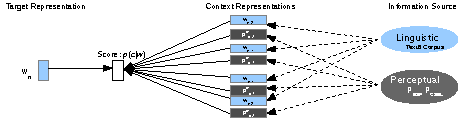
\includegraphics[width = \textwidth]{Chapter_3/Figure_1_EMNLP2014}  \caption{Our multi-modal model architecture. Light boxes are elements of the original \cite{mikolov2013efficient} model. For target words \(w_n\) in the domain of \(\mathbf{P}\), the model updates based on corpus context words \( w_{n+i} \) then on words \(p^w_{n+i}\) in perceptual psuedo-sentences. Otherwise, updates are based solely on the \( w_{n+i}. \)}\end{figure*}

For each word type \(w\) in the vocabulary \(V\), the model learns both a `target-embedding' \( r_{w} \in \mathbb{R}^d\) and a `context-embedding' \(\hat{r}_{w} \in \mathbb{R}^d\) such that, given a target word, its ability to predict nearby context words is maximized. The probability of seeing context word \(c\) given target \(w\) is defined as:  

\[p(c|w)  = \frac{\me^{\hat{r}_{c} \cdot r_{w}}}{\sum_{v \in V} \me^{\hat{r}_v\cdot r_{w}}}    \] 

The model learns from a set of target-word, context-word pairs, extracted from a corpus of sentences as follows. In a given sentence \(S\) (of length \(N\)), for each position \( n \leq N\), each word \(w_n\) is treated in turn as a target word. An integer \( {t(n)} \) is then sampled from a uniform distribution on \( \{1, \dots k \} \), where \(k > 0\) is a predefined maximum context-window parameter. The pair tokens \( \{(w_n, w_{n+j}): -{t(n)}\leq j \leq {t(n)}, w_i \in S \}\) are then appended to the training data. Thus, target/context training pairs are such that (i) only words within a \(k\)-window of the target are selected as context words for that target, and (ii) words closer to the target are more likely to be selected than those further away.

The training objective is then to maximize the log probability \( T\) across of all such examples from \(S\), and then across all sentences in the corpus:
 
\[ T = \frac{1}{N} \sum_{n=1}^{N} \sum_{-{t(n)}\leq j \leq {t(n)}, j\neq 0} log(  p(w_{n+j}|w_{n}) ) \]The model free parameters (target-embeddings and context-embeddings of dimension \(d\) for each word in the corpus with frequency above a certain threshold \(f\)) are updated according to stochastic gradient descent and backpropation, with learning rate controlled by Adagrad \cite{duchi2011adaptive}. For efficiency, the output layer is encoded as a hierarchical softmax function based on a binary Huffman tree \cite{morin2005hierarchical}. 

As with other distributional architectures, the model captures conceptual semantics by exploting the fact that words appearing in similar linguistic contexts are likely to have similar meanings. Informally, the model adjusts its embeddings to increase the `probability' of seeing the language in the training corpus. Since this probability increases with the \(p(c|w)\), and the \(p(c|w)\) increase with the dot product \( \hat{r}_v\cdot r_{c} \), the updates have the effect of moving each target-embedding incrementally `closer' to the context-embeddings of its collocates. In the target-embedding space, this results in embeddings of concept words that regularly occur in similar contexts moving closer together.   


\paragraph{Multi-modal Extension} We extend the \cite{mikolov2013efficient} architecture via a simple means of introducing perceptual information that aligns with human language learning. Based on the assumption that frequency in domain-general linguistic corpora correlates with the likelihood of `experiencing' a concept in the world \cite{bybee2001frequency,chater2006probabilistic}, perceptual information is introduced to the model whenever designated concrete concepts are encountered in the running-text linguistic input. This has the effect of introducing more perceptual input for commonly experienced concrete concepts and less input for rarer concrete concepts. 

To implement this process,  perceptual information is extracted from external sources and encoded in an associative array \(\bf{P}\), which maps (typically concrete) words \(w\) to bags of perceptual features \({\bf b}(w)\). The construction of this array depends on the perceptual information source; the process for our chosen sources is detailed in Section~\ref{percep_sources}.  

Training our model begins as before on running-text. When a sentence \(S_m\) containing a word \(w\) in the domain of \(\mathbf{P}\) is encountered, the model completes training on \(S_m\) and begins learning from a perceptual pseudo-sentence \(\hat{S}(w)\).  \(\hat{S_m}(w)\) is constructed  by randomly sampling features from \({\bf b}(w)\) to occupy positions before and instances of \(w\), so that  \(\hat{S_m}(w)\) is the same length as \(S_m\) (see Figure~\ref{examples}). Once training on \(\hat{S_m}(w)\) is completed, the model reverts to the next `real' (linguistic) sentence \(S_{m+1}\), and the process continues. Thus, when a concrete concept is encountered in the corpus, its embedding is first updated based on language (moved incrementally closer to concepts appearing in similar linguistic contexts), and then on perception (moved incrementally closer to concepts with the same or similar perceptual features).  

For greater flexibility, we introduce a parameter \(\alpha\) reflecting the raw quantity of perceptual information relative to linguistic input. When \(\alpha=2\), two pseudo-sentences are generated and inserted for every corpus occurrence of a token from the domain of \(\mathbf{P}\). For non-integral \(\alpha \), the number of sentences inserted is \( \lfloor \alpha \rfloor \), and a further sentence is added with probability \(\alpha - \lfloor \alpha \rfloor \).

In all experiments reported in the following sections we set the window size parameter \(k = 5\) and the minimum frequency parameter \(f = 3\), which guarantees that the model learns embeddings for all concepts in our evaluation sets. While the model learns both target and context-embeddings for each word in the vocabulary, we conduct our experiments with the target embeddings only. We set the dimension parameter \(d = 300 \) as this produces high quality embeddings in the language-only case \cite{mikolov2013efficient}. 

\begin{figure} \(\hat{S}(crocodile) =\)\small{ {\bf Crocodile} legs {\bf crocodile} teeth {\bf crocodile} teeth {\bf crocodile} scales {\bf crocodile} green {\bf crocodile}. \\ \\ \(\hat{S}(screwdriver)=\) { \bf Screwdriver} handle {\bf screwdriver} flat  {\bf screwdriver} long {\bf screwdriver}  handle {\bf screwdriver}  head. } \caption{\label{examples} Example pseudo-sentences generated by our model.}\end{figure}

\subsection{Information Sources}
\label{percep_sources}

We construct the associative array of perceptual information \(\mathbf{P}\) from two sources typical of those typically used for multi-modal semantic models.

\paragraph{ESPGame Dataset} The ESP-Game dataset (ESP) \cite{von2004labeling} consists of 100,000 images, each annotated with a list of lexical concepts that appear in that image.  

For any concept \(w\) identified in an ESP image, we construct a corresponding bag of features \({\bf b}(w)\). For each ESP image \(I\) that contains \(w\), we append the other concept tokens identified in \(I\) to \({\bf b}(w)\). Thus, the more frequently a concept co-occurs with \(w\) in images, the more its corresponding lexical token occurs in \({\bf b}(w)\). The array \(\mathbf{P_{ESP}}\) in this case then consists of the  \( (w,  {\bf b}(w) ) \) pairs.

\paragraph{CSLB Property Norms} The Centre for Speech, Language and the Brain norms (CSLB) \cite{devereux2013centre} is a recently-released dataset containing semantic properties for 638 concrete concepts produced by human annotators. The CSLB dataset was compiled in the same way as the \cite{mcrae2005semantic} property norms used widely in multi-modal models \cite{silberer2012grounded,rollermultimodal}; we use CSLB because it contains more concepts. For each concept, the proportion of the 30 annotators that produced a given feature can also be employed as a measure of the strength of that feature.

When encoding the CSLB data in \(\mathbf{P}\), we first map properties to lexical forms (e.g. \emph{is\_green} becomes \emph{green}). By directly identifying perceptual features and linguistic forms in this way, we treat features observed in the perceptual data as (sub)concepts to be acquired via the same multi-modal input streams and stored in the same domain-general memory as the evaluation concepts. This design decision in fact corresponds to a view of cognition that is sometimes disputed \cite{fodor1983modularity}. In future studies we hope to compare the present approach to architectures with domain-specific conceptual memories. 

For each concept \(w\) in CSLB, we then construct a feature bag \({\bf b}(w)\) by appending lexical forms to \({\bf b}(w)\) such that the count of each feature word is equal to the strength of that feature for \(w\). Thus, when features are sampled from \({\bf b}(w)\) to create pseudo-sentences (as detailed previously) the probability of a feature word occuring in a sentence reflects feature strength. The array \(\mathbf{P_{CSLB}}\) then consists of all \( (w,  {\bf b}(w) ) \) pairs.

\paragraph{Linguistic Input} The linguistic input to all models is the 400m word Text8 Corpus\footnote{From http://mattmahoney.net/dc/textdata.html} of Wikipedia text, split into sentences and with punctuation removed. 



 \begin{table}[t]\begin{center}\begin{tabular}{c|ccc|c}


\multicolumn{2}{c}{\bf ESPGame} &\multicolumn{1}{c}{} & \multicolumn{2}{c}{\bf CSLB}\\
 \underline{Image 1} &  \underline{Image 2} & &  \underline{Crocodile} & \underline{Screwdriver} \\ 
\footnotesize{red} &  \footnotesize{wreck} &  &  \footnotesize{has 4 legs (7)} &  \footnotesize{has handle (28)} \\ 
\footnotesize{chihuaua} &  \footnotesize{cyan} & &  \footnotesize{has tail (18)} &  \footnotesize{has head (5)} \\ 
\footnotesize{eyes} &  \footnotesize{man} & &  \footnotesize{has jaw (7)} & \footnotesize{is long (9)} \\ 
\footnotesize{little} &  \footnotesize{crash} & &  \footnotesize{has scales (8)} &   \footnotesize{is plastic (18)} \\ 
\footnotesize{ear} &  \footnotesize{accident} & &  \footnotesize{has teeth (20)} & \footnotesize{is metal (28)} \\ 
\footnotesize{nose}  &  \footnotesize{street} & &  \footnotesize{is green (10}) &  \\ 
\footnotesize{small} &   & & \footnotesize{is large (10)} &    \\ 






\end{tabular}\end{center}\caption{\label{font-table} Concepts identified in images in the ESP Game (left) and features produced for concepts by human annotators in the CSLB dataset (with feature strength, max=30).}\end{table}







\subsection{Evaluation}

We evaluate the quality of representations by how well they reflect \emph{free association} scores, an empirical measure of cognitive conceptual proximity. The University of South Florida Norms (USF) \cite{nelson2004university} contain free association scores for over 40,000 concept pairs, and have been widely used in NLP to evaluate semantic representations \cite{andrews2009integrating,feng2010visual,silberer2012grounded,rollermultimodal}. Each concept that we extract from the USF database has also been rated for conceptual concreteness on a Likert scale of 1-7 by at least 10 human annotators. Following previous studies \cite{huang2012improving,silberer2012grounded}, we measure the (Spearman \(\rho\)) correlation between association scores and the cosine similarity of vector representations.

 \begin{table}[t]\begin{center}\begin{tabular}{l|l|c}



\bf Concept 1 & \bf Concept 2 & \bf Assoc. \\
 \hline 
abdomen \footnotesize{ (6.83)} & stomach \footnotesize{ (6.04)} & 0.566 \\
throw \footnotesize{  (4.05)} & ball  \footnotesize{ (6.08)} & 0.234 \\
hope \footnotesize{  (1.18)} & glory \footnotesize{ (3.53)} & 0.192 \\
egg \footnotesize{ (5.79)} & milk \footnotesize{ (6.66)} & 0.012 \\



\end{tabular}\end{center}\caption{\label{font-table} Example concept pairs (with mean concreteness rating) and free-association scores from the USF dataset.}\end{table}






We create separate abstract and concrete concept lists by ranking the USF concepts according to concreteness and sampling at random from the first and fourth quartiles. We also introduce a complementary noun/verb dichotomy,\footnote{Based on the majority POS-tag of words in the lemmatized British National Corpus \cite{leech1994claws4}} on the intuition that information propagation may occur differently from noun to noun or from noun to verb (because of their distinct structural relationships in sentences). The abstract/concrete and noun/verb dichotomies yield four distinct concept lists. For consistency, the concrete noun list is filtered so that all concrete noun concepts \(w\) have perceptual representations {\bf b}(w) in both  \(\mathbf{P_{ESP}}\) and  \(\mathbf{P_{CSLB}}\). For each of the four resulting concept lists \(C\) (concrete/abstract, noun/verb), a corresponding set of evaluation pairs  \( \{ (w_1, w_2) \in USF :  w_1, w_2 \in C\}\) is extracted (see Table 3 for details). 



 \begin{table}[t]\begin{center}\begin{tabular}{l|r|r|p{2.1cm}}



\bf Concept Type & \bf  List & \bf Pairs & \bf Examples \\ 

\hline concrete nouns & 541 & 1418 & \emph{yacht, cup} \\

abstract nouns & 100 & 295 & \emph{fear, respect} \\

all nouns & 666 & 1815 & \emph{fear, cup} \\

concrete verbs & 50 & 66 & \emph{kiss, launch} \\

abstract verbs & 50 & 127 & \emph{differ, obey} \\

all verbs & 100 & 221 & \emph{kiss, obey} \\

\end{tabular}\end{center}\caption{\label{font-table} Details the subsets of USF data used in our evaluations, downloadable from our website.}\end{table}






\subsection{Results and Discussion}

Our experiments were designed to answer four questions, outlined in the following subsections: (1) Which model architectures perform best at \emph{combining} information pertinent to multiple modalities when such information exists explicitly (as common for concrete concepts)? (2) Which model architectures best propagate perceptual information to concepts for which it does not exist explicitly (as is common for abstract concepts)? (3) Is it preferable to include all of the perceptual input that can be obtained from a given source, or to filter this input stream in some way? (4) How much perceptual vs. linguistic input is optimal for learning various concept types? 

\subsection{Combining information sources} To evaluate our approach as a method of information combination we compared its performance on the concrete noun evaluation set against alternative methods. When implementing the alternatives, we first encoded the perceptual input directly into sparse feature vectors, with coordinates for each of the 2726 features in CSLB and for each of the 100,000 images in ESP. 

The first alternative is simple concatenation of these perceptual vectors with linguistic vectors embeddings learned by the \cite{mikolov2013efficient} model on the Text8 Corpus. In the second alternative, proposed for multi-modal models by \cite{silberer2012grounded}, \emph{canonical correlation analysis} (CCA) \cite{hardoon2004canonical} was applied to the vectors of both modalities. This yields reduced-dimensionality representations that preserve underlying inter-modal correlations, which are then concatenated. The final alternative, proposed by \cite{bruni2014multimodal} involves applying Singular Value Decomposition (SVD) to the matrix of concatenated multi-modal representations, yielding smoothed representations.\footnote{CCA was implemented using the \emph{CCA} package in R. SVD was implemented using the Python \emph{sparsesvd} package, with truncation factor \(k=1024\) as per \cite{bruni2014multimodal}.}



We compare these alternatives to our proposed model with \(\alpha = 1\). In The CSLB and ESP models, all training pseudo-sentences are generated from the arrays \(\mathbf{P_{CSLB}}\) and \(\mathbf{P_{ESP}}\) respectively. In the models classed as \emph{CSLB\&ESP}, a random choice between \(\mathbf{P_{CSLB}}\) and \(\mathbf{P_{ESP}}\) is made every time perceptual input is included (so that the overall quantity of perceptual information is the same). 

As shown in Figure~\ref{main_results} (left side), the embeddings learned by our model achieve a higher correlation with the USF data than simple concatenation, CCA and SVD regardless of perceptual input source. With the optimal perceptual source (ESP only), for instance, the correlation is 11\% higher that the next best alternative method, CCA. 

One possible factor behind this improvement is that, in our model, the learned representations fully integrate the two modalities, whereas for both CCA and the concatenation method each representation feature (whether of reduced dimension or not) corresponds to a particular modality. This deeper integration may help our architecture to overcome the challenges inherent in information combination such as inter-modality differences in information content and representation sparsity.   


\subsection{Propagating input to abstract concepts}To test the process of information propagation in our model, we evaluated the learned embeddings of more abstract concepts. We compared our approach with two recently-proposed alternative methods for inferring perceptual features when explicit perceptual information is unavailable. 

\paragraph{Johns and Jones}In the method of \cite{johns2012perceptual}, pseudo-perceptual representations for target concepts without a perceptual representations (uni-modal concepts) are inferred as a weighted average of the perceptual representations of concepts that do have such a representation (bi-modal concepts). 

In the first step of their two-step method, for each uni-modal concept  \(\bf k\), a quasi-perceptual representation is computed as an average of the perceptual representations of bi-modal concepts, weighted by the proximity between each of these concepts and \( \bf k\)\[{\bf k}^p = \sum_{{\bf c} \in \bar{C}} S({\bf k}^l,{\bf c}^l)^\lambda \cdot {\bf c}^p  \] where \(  \bar{C} \) is the set of bi-modal concepts, \({\bf c}^p\) and  \({\bf k}^p\) are the perceptual representations for \(\bf c\) and \(\bf k\) respectively, and  \({\bf c}^l\) and \({\bf k}^l\) the linguistic representations. The exponent parameter \(\lambda \) reflects the learning rate. 

In step two, the initial quasi-perceptual representations are inferred for a second time, but with the weighted average calculated over the perceptual or initial quasi-perceptual representations of all other words, not just those that were orignally bi-modal. As with \cite{johns2012perceptual}, we set the learning rate parameter \( \lambda\) to be 3 in the first step and 13 in the second.  


\paragraph{Ridge Regression}An alternative, proposed for the present purpose by [ref. withdrawn for review], uses \emph{ridge regression} \cite{myers1990classical}. Ridge regression is a variant of least squares regression in which a regularization term is added to the training objective to favor solutions with certain properties. 

For bi-modal concepts of dimension \(n_p\), we apply ridge regression to learn \(n_p\) linear functions \( f_i: \mathbb{R}^{n_l} \to \mathbb{R} \) that map the linguistic representations (of dimension \(n_l\)) to a particular perceptual feature \(i\). These functions are then applied together to map the linguistic representations of uni-modal concepts to full quasi-perceptual representations.

Following [ref. withdrawn for review], we take the Euclidian \( l_2 \) norm of the inferred parameter vector as the regularization term. This ensures that the regression favors lower coefficients and a smoother solution function, which should provide better generalization performance than simple linear regression. The objective for learning the \( f_i \) is then to minimize \[ \| {\bf a}X - Y_i \|_2^2 + \|{\bf a}\|_2^2 \]where \( {\bf a}\) is the vector of regression coefficients, \( X \) is a matrix of linguistic representations and \(  Y_i \) a vector of the perceptual feature \(i\) for the set of bi-modal concepts.

\paragraph{Comparisons}We applied the Johns and Jones method and ridge regression starting from linguistic embeddings acquired by the \cite{mikolov2013efficient} model on the Text8 Corpus, and concatenated the resulting pseudo-perceptual and linguistic representations. As with the implementation of our model, the perceptual input for these alternative models was limited to concrete nouns (i.e. concrete nouns were the only bi-modal concepts in the models).

 \begin{figure*}  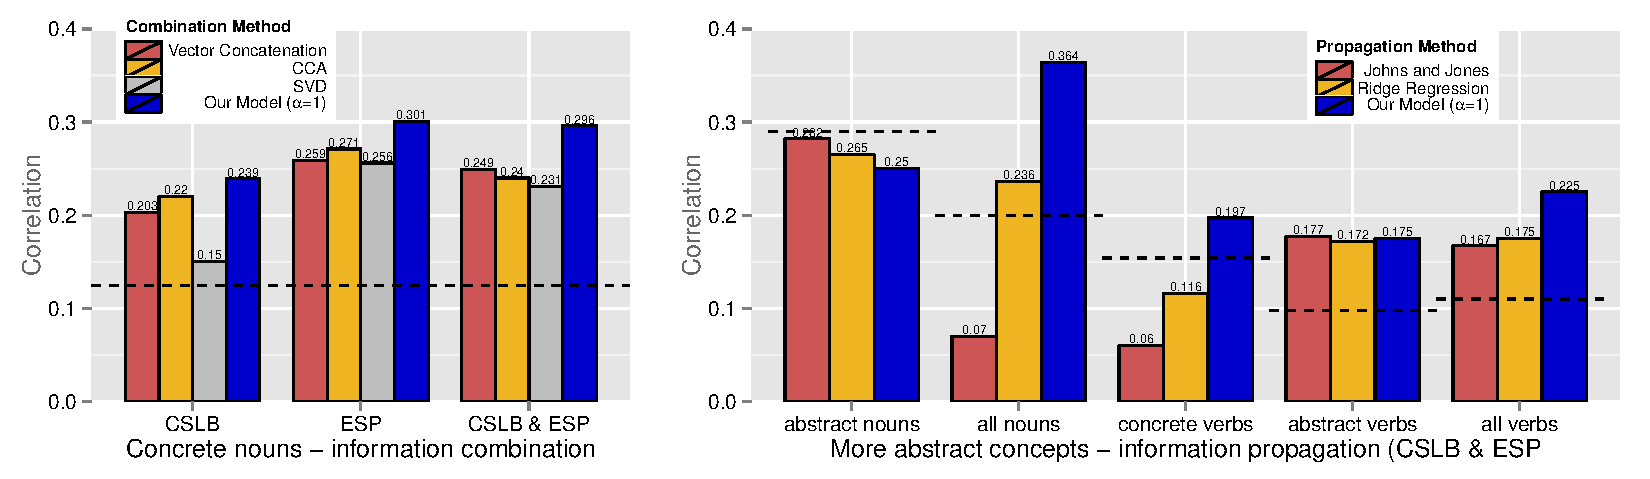
\includegraphics[width = \textwidth]{Chapter_3/Graph_1_EMNLP2014}  \caption{\label{main_results} The proposed approach compared with other methods of information combination (left) and propagation. Dashed lines indicate language-only model baseline.}\end{figure*}

Figure~\ref{main_results} (right side) illustrates the propagation performance of the three models. While the correlations overall may seem somewhat low, this is a consequence of the difficulty of modeling the USF data. In fact, the performance of both the language-only model and our multi-modal extension across the concept types, ranging from .18--.36, is equal to or higher than equivalent models evaluated on the same data previously \cite{feng2010visual,silberer2012grounded,silberer2013models}. 

For learning representations of concrete verbs, our approach achieves a 69\% increase in performance over the next best alternative. The performance of the model on abstract verbs is marginally inferior to Johns and Jones' method. Nevertheless, the clear advantage for concrete verbs makes our model the best choice for learning representations of verbs in general, as shown by performance on the set \emph{all verbs}, which also includes mixed abstract-concrete pairs. 

Our model is also marginally inferior to alternative approaches in learning representations of abstract nouns. However, in this case, no method improves on the linguistic-only baseline. It is possible that perceptual information is simply so removed from the core semantics of these concepts that they are best acquired via the linguistic medium alone, regardless of learning mechanism. The moderately inferior performance of our method in such cases is likely caused by its greater inherent inter-modal dependence compared with methods that simply concatenate uni-modal representations. When the perceptual signal is of low quality, this greater inter-modal dependence allows the linguistic signal to be obscured. The trade-off, however, is the higher quality joint representations when the perceptual signal is of higher-quality, exemplified by the fact that our proposed approach outperforms alternatives on the set \emph{all nouns}, which includes the more concrete nouns. 

\subsection{Direct representation vs. propagation}

 \begin{figure*}[t] 

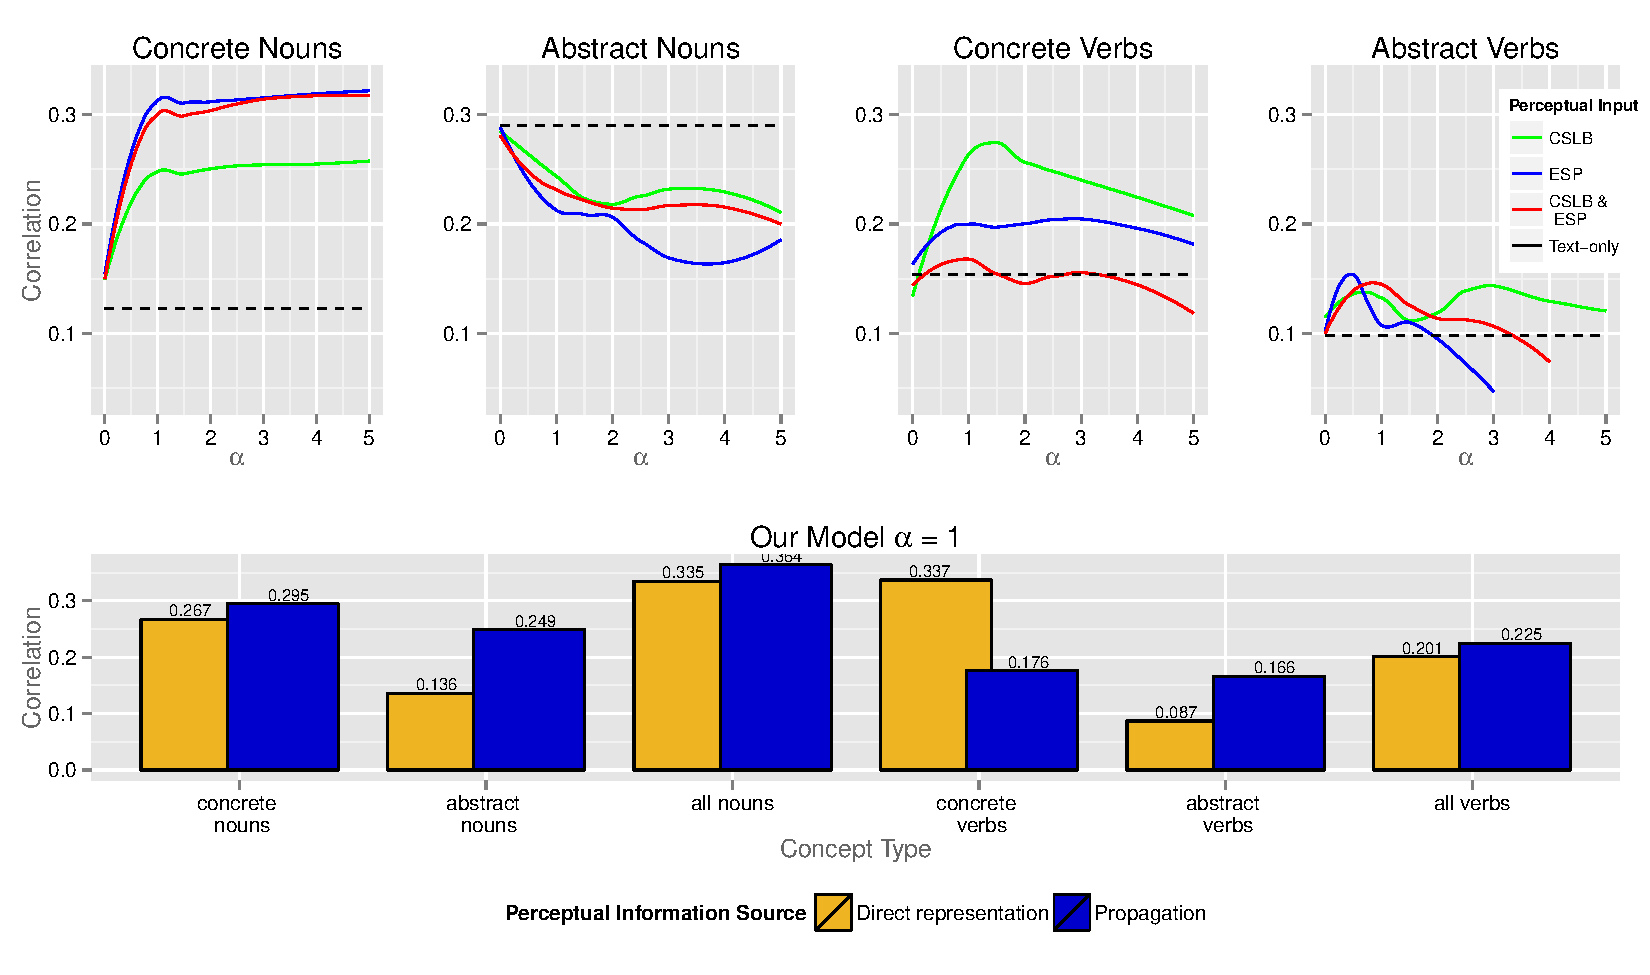
\includegraphics[width = \textwidth]{Chapter_3/Graph_2_EMNLP2014}  

\caption{\label{repprop} Top: Comparing the strategy of directly representing abstract concepts from perceptual information where available (yellow bars) vs. propagating via concrete concepts. Bottom: The effect of increasing \(\alpha\) on correlation with USF pairs (Spearman \(\rho\)) for each concept type. Horizontal dashed lines indicate language-only model baseline.}

\end{figure*}

Although property norm datasets such as the CSLB data typically consist of perceptual feature information for concrete nouns only, image-based datasets such as ESP do contain information on more abstract concepts, which was omitted from the previous experiments. Indeed, image banks such as Google Images contain millions of photographs portraying quite abstract concepts, such as \emph{love} or \emph{war}. On the other hand, encodings or descriptions of abstract concepts are generally more subjective and less reliable than those of concrete concepts \cite{katja2005content}. We therefore investigated whether or not it is preferable to include this additional information as model input or to restrict perceptual input to concrete nouns as previously.    

Of our evaluation sets, it was possible to construct from ESP (and add to \(\mathbf{P_{ESP}}\)) representations for all of the concrete verbs, and for approximately half of the abstract verbs and abstract nouns. Figure~\ref{repprop} (top), shows the performance of a our model trained on all available perceptual input versus the model in which the perceptual input was restricted to concrete nouns. 

The results reflect a clear manifestation of the abstract/concrete distinction. Concrete verbs behave similarly to concrete nouns, in that they can be effectively represented directly from perceptual information sources. The information encoded in these representations is beneficial to the model and increases performance. In contrast, constructing `perceptual' representations of abstract verbs and abstract nouns directly from perceptual information sources is clearly counter-productive (to the extent that performance also degrades on the combined sets \emph{all nouns} and \emph{all verbs}). It appears in these cases that the perceptual input acts to obscure or contradict the otherwise useful signal inferred from the corpus.

As shown in the previous section, the inclusion of any form of perceptual input inhibits the learning of abstract nouns. However, this is not the case for abstract verbs. Our model learns higher quality representations of abstract verbs when perceptual input is restricted to concrete nouns than when no perceptual input is included whatsoever \emph{and} when perceptual input is included for both concrete nouns and abstract verbs. This supports the idea of a gradual scale of concreteness: the most concrete concepts can be effectively represented directly in the perceptual modality; somewhat more abstract concepts cannot be represented directly in the perceptual modality, but have representations that are improved by propagating perceptual input from concrete concepts via language; and the most abstract concepts are best acquired via language alone.   

\subsection{Source and quantity of perceptual input} For different concept types, we tested the effect of varying the proportion of perceptual to linguistic input (the parameter \(\alpha\)). Perceptual input was restricted to concrete nouns as in Sections 3.1-3.2. 

As shown in Figure~\ref{repprop}, performance on concrete nouns improves (albeit to a decreasing degree) as \( \alpha \) increases. When learning concrete noun representations, linguistic input is apparently redundant if perceptual input is of sufficient quality and quantity. For the other concept types, in each case there is an optimal value for \( \alpha \) in the range .5--2, above which perceptual input obscures the linguistic signal and performance degrades. The proximity of these optima to 1 suggests that  for optimal learning, when a concrete concept is experienced approximately equal weight should be given to available perceptual and linguistic information. 

\subsection{Conclusions}

Motivated by the notable prevalence of abstract concepts in everyday language, and their likely importance to flexible, general-purpose representation learning, we have investigated how abstract and concrete representations can be acquired by multi-modal models. In doing so, we presented a simple and easy-to-implement architecture for acquiring semantic representations of both types of concept from linguistic and perceptual input. 

While neuro-probabilistic models have been applied to the problem of multi-modal representation learning previously \cite{srivastava2012multimodal,wu2013online} our model and experiments develop this work in several important ways. First, we address the problem of learning abstract concepts. By isolating concepts of different concreteness and part-of-speech in our evaluation sets, and separating the processes of information combination and propagation, we demonstrate that the multi-modal approach is indeed effective for some, but perhaps not all, abstract concepts. In addition, our model introduces a clear parallel with human language learning. Perceptual input is introduced precisely when concrete concepts are `experienced' by the model in the corpus text, much like a language learner experiencing concrete entities via sensory perception.  

Taken together, our findings indicate the utility of distinguishing three concept types when learning representations in the multi-modal setting. 

\paragraph{Type I}Concepts that can be effectively represented directly in the perceptual modality. For such concepts, generally concrete nouns or concrete verbs, our proposed approach provides a simple means of combining perceptual and linguistic input. The resulting multi-modal representations are of higher quality than those learned via other approaches, resulting in a performance improvement of over 10\% in modelling free association.

\paragraph{Type II}Concepts, including abstract verbs, that cannot be effectively represented directly in the perceptual modality, but whose representations can be improved by joint learning from linguistic input and perceptual information about related concepts. Our model can effectively propagate perceptual input (exploiting the relations inferred from the linguistic input) from Type I concepts to enhance the representations of Type II concepts above the language-only baseline. Because of the frequency of abstract concepts, such propagation extends the benefit of the multi-modal approach to a far wider range of language than models based solely in the concrete domain. 

\paragraph{Type III}Concepts, such as abstract nouns, which are more effectively learned via language-only models than multi-modal models. Neither the model we introduce here nor other proposed propagation methods achieve an improvement in representation quality for these concepts over the language-only baseline. Of course, it is an empirical question whether a multi-modal approach could ever enhance the representation learning of these concepts, one with potential implications for cognitive theories of grounding (a topic of much debate in psychology \cite{grafton2009embodied,barsalou2010grounded}). 

Additionally, we investigated the optimum type and quantity of perceptual input for learning concepts of different types. We showed that too much perceptual input can result in degraded representations. For concepts of type I and II, the optimal quantity resulted from setting \(\alpha = 1\); i.e. whenever a concrete concept was encountered, the model learned from an equal number of language-based and perception-based examples. While we make no formal claims here, such observations may ultimately provide insight into human language learning and semantic memory. 

In future we will address the question of whether Type III concepts can ever be enhanced via multi-modal learning, and investigate multi-modal models that optimally learn concepts of each type. This may involve filtering the perceptual input stream for concepts according to concreteness, and possibly more elaborate model architectures that facilitate distinct representational frameworks for abstract and concrete concepts.

 \section{Multi-modal fusion based on image dispersion}




\section{Improving the Evaluation of Word Representations}

There is very little similar about coffee and cups. \emph{Coffee} refers to a plant, which is a living organism or a hot brown (liquid) drink. In contrast, a \emph{cup} is a man-made solid of broadly well-defined shape and size with a specific function relating to the consumption of liquids. Perhaps the only clear trait these concepts have in common is that they are concrete entities. Nevertheless, in what is currently the most popular evaluation gold standard for semantic similarity, WordSim(WS)-353 \cite{finkelstein2001placing}, \emph{coffee} and \emph{cup} are rated  as more `similar' than pairs such as \emph{car} and \emph{train}, which share numerous common properties (function, material, dynamic behaviour, wheels, windows etc.). Such anomalies also exist in other gold standards such as the MEN dataset \cite{bruni2012distributional}. As a consequence, these evaluations effectively penalise models for learning the evident truth that \emph{coffee} and \emph{cup} are dissimilar. 

Although clearly different, \emph{coffee} and \emph{cups} are very much related. The psychological literature refers to the conceptual relationship between these concepts as \emph{association}, although it has been given a range of names including \emph{relatedness} \cite{budanitsky2006evaluating,agirre2009study}, \emph{topical similarity} \cite{hatzivassiloglou2001simfinder} and \emph{domain similarity} \cite{turney2012domain}. Association contrasts with \emph{similarity}, the relation connecting \emph{cup} and \emph{mug} \cite{tversky1977features}. At its strongest, the similarity relation is exemplified by pairs of \emph{synonyms}; words with identical referents.

Computational models that effectively capture similarity as distinct from association have numerous applications. Such models are used for the automatic generation of dictionaries, thesauri, ontologies and language correction tools \cite{cimiano2005learning,biemann2005ontology,li2006exploring}. Machine translation systems, which aim to define mappings between fragments of different languages whose meaning is similar, but not necessarily associated, are another established application \cite{he2008indirect,marton2009improved}. Moreover, since, as we establish, similarity is a cognitively complex operation that can require rich, structured conceptual knowledge to compute accurately, similarity estimation constitutes an effective proxy evaluation for general-purpose representation-learning models whose ultimate application is variable or unknown \cite{collobert2008unified,baroni2010distributional}.

As we show in Section 2, the predominant gold standards for semantic evaluation in NLP do not measure the ability of models to reflect similarity. In particular, in both WS-353 and MEN, pairs of words with associated meaning, such as \emph{coffee} and \emph{cup} (rating = 6.8) \emph{telephone} and \emph{communication} (7.5) or \emph{movie} and \emph{theater} (7.7), receive a high rating regardless of whether or not their constituents are similar. Thus, the utility of such resources to the development and application of similarity models is limited, a problem exacerbated by the fact that many researchers appear unaware of what their evaluation resources actually measure.\footnote{For instance,  \cite{huang2012improving} (pages 1,4,10) and \cite{reisinger2010multi} (page 4) refer to MEN and/or WS-353 as `similarity datasets'. Others evaluate on both these association-based and genuine similarity-based gold standards with no reference to the fact that they measure different things \cite{medelyan2009mining,li2014obtaining}.} 

While certain smaller gold standards, those of \cite{rubenstein1965contextual} (RG) and \cite{agirre2009study} (WS-Sim), do focus clearly on similarity, these resources suffer from other important limitations. For instance, as we show, and as is also the case for WS-353 and MEN, state-of-the-art models have reached the average performance of a human annotator on these evaluations. It is common practice in NLP to define the upper limit for automated performance on an evaluation as the average human performance or inter-annotator agreement \cite{yong1999case,cunningham2005information,resnik201011}. Based on this established principle and the current evaluations, it would therefore be reasonable to conclude that the problem of representation learning, at least for similarity modelling, is approaching resolution. However, circumstantial evidence suggests that distributional models are far from perfect. For instance, we are some way from automatically-generated dictionaries, thesauri or ontologies that can be used with the same confidence as their manually-created equivalents.   

Motivated by these observations, in Section 3 we present \emph{SimLex-999}, a gold standard resource for evaluating the ability of models to reflect similarity. SimLex-999 was produced by 500 paid native English speakers, recruited via Amazon Mechanical Turk,\footnote{\url{www.mturk.com/}} who were asked to rate the similarity, as opposed to association, of concepts via a simple visual interface. The choice of evaluation pairs in SimLex-999 was motivated by empirical evidence that humans represent concepts of distinct part-of-speech (POS) \cite{gentner1978relational} and conceptual concreteness \cite{hill2013quantitative} differently. While existing gold standards contain only concrete noun concepts (MEN) or cover only some of these distinctions via a random selection of items (WS-353, RG), SimLex-999 contains a principled selection of adjective, verb and noun concept pairs covering the full concreteness spectrum. This design enables more nuanced analyses of how computational models overcome the distinct challenges of representing concepts of these types. 

In Section 4 we present quantitative and qualitative analyses of the SimLex-999 ratings, which indicate that participants found it unproblematic to quantify consistently the similarity of the full range of concepts and to distinguish it from association. Unlike existing datasets, SimLex-999 therefore contains a significant number of pairs, such as [\emph{movie}, \emph{theater}], which are strongly associated but receive low similarity scores.   

The second main contribution of this paper, presented in Section 5, is the evaluation of state-of-the-art distributional semantic models using SimLex-999. These include the well known neural language models (NLMs) of \cite{huang2012improving}, \cite{collobert2008unified} and \cite{mikolov2013efficient}, which we compare with traditional vector-space co-occurrence models (VSMs) \cite{turney2010frequency} with and without dimensionality reduction (SVD) \cite{landauer1997solution}. Our analyses demonstrate how SimLex-999 can be applied to uncover substantial differences in the ability of models to represent concepts of different types. 

Despite these differences, the models we consider each share the characteristic of being better able to capture association than similarity. We show that the difficulty of estimating similarity is driven primarily by those strongly-associated pairs with a high (association) rating in gold standards such as WS-353 and MEN, but a low similarity rating in SimLex-999. As a result of including these challenging cases, together with a wider diversity of lexical concepts in general, current models achieve notably lower scores on SimLex-999 than on existing gold standard evaluations, and well below the SimLex-999 inter-human agreement ceiling. 

Finally, we explore ways in which distributional models might improve on this performance in similarity modelling. To do so, we evaluate the models on the SimLex-999 subsets of adjectives, nouns and verbs, as well as on abstract and concrete subsets and subsets of more and less strongly associated pairs (Sections 5.2.2-5.2.4). As part of these analyses, we confirm the hypothesis \cite{agirre2009study,levy2014dependency} that models learning from input informed by dependency parsing, rather than simple running-text input, yield improved similarity estimation and, specifically, clearer distinction between similarity and association. In contrast, we find no evidence for a related hypothesis \cite{agirre2009study,kiela2014systematic}, that smaller context windows improve the ability of models to capture similarity. We do, however, observe clear differences in model performance on the distinct concept types included in SimLex-999. Taken together, these experiments demonstrate the benefit of the diversity of concepts included in SimLex-999; it would not have been possible to derive similar insights by evaluating on existing gold standards.

We conclude by discussing how observations such as these can guide future research into distributional semantic models. By facilitating better-defined evaluations and finer-grained analyses, we hope that SimLex-999 will ultimately contribute to the development of models that accurately reflect human intuitions of similarity for the full range of concepts in language. 

\section{Design Motivation}

In this section, we motivate the design decisions made in developing SimLex-999. We begin (2.1) by examining the distinction between similarity and association. We then show that for a meaningful treatment of similarity it is also important to take a principled approach to  both part-of-speech (POS) and conceptual concreteness (2.2). We finish by reviewing existing gold standards, and show that none enables a satisfactory evaluation of the capability of models to capture similarity (2.3).

\subsection{Similarity and Association}

The difference between association and similarity is exemplified by the concept pairs [\emph{car, bike}] and [\emph{car, petrol}]. \emph{Car} is said to be (semantically) similar to \emph{bike} and associated with (but not similar to) \emph{petrol}. Intuitively, \emph{car} and \emph{bike} can be understood as similar because of their common physical features (e.g. wheels), their common function (transport), or because they fall within a clearly definable category (modes of transport). In contrast, \emph{car} and \emph{petrol} are associated because they frequently occur together in space and language, in this case as a result of a clear functional relationship \cite{plaut1995semantic,mcrae2012semantic}. 

Association and similarity are neither mutually exclusive nor independent. \emph{Bike} and \emph{car}, for instance, are related to some degree by both relations. Since it is common in both the physical world and in language for distinct entities to interact, it is relatively easy to conceive of concept pairs, such as \emph{car} and \emph{petrol}, that are strongly associated but not similar. Identifying pairs of concepts for which the converse is true is comparatively more difficult. One exception is common concepts paired with low frequency synonyms, such as \emph{camel} and \emph{dromedary}. Since the essence of association is co-occurrence (linguistic or otherwise \cite{mcrae2012semantic}), such pairs can seem, at least intuitively, to be similar but not strongly associated.  

To explore the interaction between the two cognitive phenomena quantitatively, we exploited perhaps the only two existing large-scale means of quantifying similarity and association. To estimate similarity, we considered proximity in the WordNet taxonomy \cite{fellbaum1999wordnet}. Specifically, we applied the measure of \cite{wu1994verbs} (henceforth \emph{WupSim}), which approximates similarity on a [0,1] scale reflecting the minimum distance between any two synsets of two given concepts in WordNet. WupSim has been shown to correlate well with human judgements on the similarity-focused RG dataset \cite{wu1994verbs}. To estimate association, we extracted ratings directly from the University of South Florida Free Association Database (USF) \cite{nelson2004university}. These data were generated by presenting human subjects with one of 5000 cue concepts and asking them to write the \emph{first word that comes into their head that is associated with or meaningfully related to that concept}. Each cue concept \( c \) was normed in this way by over 10 participants, resulting in a set of associates for each cue, and a total of over 72,000 \((c,a)\) pairs. Moreover, for each such pair, the proportion of participants who produced associate \(a\) when presented with cue \(c\) can be used as a proxy for the strength of association between the two concepts.

By measuring WupSim between all pairs in the USF dataset, we observed, as expected, a high correlation between similarity and association strength across all USF pairs (Spearman \( \rho= 0.65, p<0.001 \)). However, in line with the intuitive ubiquity of pairs such as \emph{car} and \emph{petrol}, of the USF pairs (all of which are associated to a greater or lesser degree) over 10\% had a WupSim score of less than 0.25. These include pairs of ontologically different entities with a clear functional relationship in the world [\emph{refrigerator, food}], which may be of differing concreteness [\emph{lung, disease}], pairs in which one concept is a small concrete part of a larger abstract category [\emph{sheriff, police}], pairs in a relationship of modification or subcategorization [\emph{gravy, boat}] and even those whose principal connection is phonetic [\emph{wiggle, giggle}]. As we show in Section 2.2, these are precisely the sort of pairs that are not contained in existing evaluation gold standards. Table 1 lists the USF noun pairs with the lowest similarity scores overall, and also those with the largest additive discrepancy between association strength and similarity.

\begin{table}[t]\begin{center}\begin{tabular}{l|l|r|r}
Concept 1 & Concept 2 & USF & WupSim \\
\hline \emph{hatchet} & \emph{murder} & 0.013 & 0.091 \\
\emph{robbery} & \emph{jail} & 0.020 & 0.100 \\
\emph{lung} & \emph{disease} & 0.014 & 0.105 \\
\emph{burglar} & \emph{robbery}& 0.020 & 0.105\\
\hdashline \emph{sheriff} & \emph{police} & 0.333 & 0.133 \\
\emph{colonel} & \emph{army} & 0.303 & 0.111 \\
\emph{quart}& \emph{milk} & 0.462 & 0.235 \\
\emph{refrigerator} & \emph{food} & 0.424 & 0.235\\
\end{tabular}\end{center}\caption{\label{font-table} Top: Concept pairs with the lowest WupSim scores in the USF dataset overall. Bottom: Pairs with the largest discrepancy in rank between association strength (high) and WupSim (low).}\end{table}

%To test the hypothesis that this interaction is asymmetric, we extracted four subsets of the USF pairs: the lowest and highest quartiles %according to similarity and the lowest and highest quartiles according to association. On each of these subsets, we re-evaluated the %correlation between similarity and association. As Figure 1 demonstrates, knowing that two concepts are similar makes it easier to %predict their association: The similarity/association correlation on the most similar pairs is clearly higher than on the least similar pairs. In %contrast, knowing that concepts are association does not make predicting their similarity easier: The correlation values for the most and %least associated pairs are roughly equal. These qualitative comparisons confirm that similarity is a stronger predictor of association than %association is of similarity. 

%\begin{figure}[ht]  \includegraphics[width =0.5\textwidth]{Figure_0}  \caption{}\end{figure}  

\subsubsection{Association and similarity in NLP} 

As noted in the Introduction, the similarity/association distinction is not only of interest to researchers in psychology or linguistics. Models of similarity are particularly applicable to various NLP tasks, such as lexical resource building, semantic parsing and machine translation \cite{he2008indirect,Haghighi2008Learning,marton2009improved,beltagysemantic}. Models of association, on the other hand, may be better suited to tasks such as word-sense disambiguation \cite{navigli2009word}, and applications such as text classification \cite{phan2008learning} in which the target classes correspond to topical domains such as \emph{agriculture} or \emph{sport} \cite{rose2002reuters}. 

Much recent research in \emph{distributional semantics} does not distinguish between association and similarity in a principled way (see e.g. \cite{huang2012improving,reisinger2010multi,luong2013better}).\footnote{Several papers that take a knowledge-based or symbolic approach to meaning do address the similarity/association issue \cite{budanitsky2006evaluating}.} One exception is \cite{turney2012domain}, who constructs two distributional models with different features and parameter settings, explicitly designed to capture either similarity or association. Using the output of these two models as input to a logistic regression classifier, Turney predicts whether two concepts are associated, similar or both, with 61\% accuracy. However, in the absence of a gold standard covering the full range of similarity ratings (rather than a list of pairs identified as being similar or not) Turney cannot confirm directly that the similarity-focused model does indeed effectively quantify similarity. 

\cite{agirre2009study} explicitly examine the distinction between association and similarity in relation to distributional semantic models. Their study is based on the partition of WS-353 into a subset focused on similarity, which we refer to as \emph{WS-Sim}, and a subset focused on association, which we term \emph{WS-Rel}. More precisely, WS-Sim is the union of the pairs in WS-353 judged by three annotators to be similar and the set \(U\) of entirely unrelated pairs, and WS-Rel is the union of \(U\) and pairs judged to be associated but not similar. Agirre et al. confirm the importance of the association/similarity distinction by showing that certain models perform relatively well on WS-Rel while others perform comparatively better on WS-Sim. However, as shown in the following section, a model need not be an exemplary model of similarity in order to perform well on WS-Sim since an important class of concept pair (associated but not similar entities) is not represented in this dataset. Therefore the insights that can be drawn from the results of the \cite{agirre2009study} study are limited.  

Several other authors touch on the similarity/association distinction in inspecting the output of distributional models \cite{andrews2009integrating,kiela2014systematic,levy2014dependency}. While the strength of the conclusions that can be drawn from such qualitative analyses is clearly limited, there appear to be two broad areas of consensus concerning similarity and distributional models: 

\begin{itemize}

\item Models that learn from input annotated for syntactic or dependency relations better reflect similarity, whereas approaches that learn from running-text or bag-of-words input better model association \cite{agirre2009study,levy2014dependency}. 

\item Models with larger context windows may learn representations that better capture association, whereas models with narrower windows better reflect similarity \cite{agirre2009study,kiela2014systematic}.

\end{itemize}







\subsection{Concepts, part-of-speech and concreteness}



Empirical studies have shown that the performance of both humans and distributional models depends on the POS category of the concepts learned. \cite{gentner2006verbs} showed that children find verb concepts harder to learn than noun concepts, and \cite{markman1997similar} present evidence that different cognitive operations are employed when comparing two nouns or two verbs. \cite{hill2014multi} demonstrate differences in the ability of distributional models to acquire noun and verb semantics. Further, they show that these differences are greater for models that learn from both text and perceptual input (as with humans).



In addition to POS category, differences in human and computational concept learning and representation have been attributed to the effects of \emph{concreteness}, the extent to which a concept has a directly perceptible physical referent. On the cognitive side, these `concreteness effects' are well established, even if the causes are still debated \cite{paivio1991dual,hill2013quantitative}. Concreteness has also been associated with differential performance in computational text-based \cite{hill2013concreteness} and multi-modal semantic models \cite{kielaimproving}.

\subsection{Existing gold standards and evaluation resources}

For brevity, we do not exhaustively review all methods that have been employed to evaluate semantic models, but instead focus on the similarity or association-based gold standards that are most commonly-applied in recent work in NLP. In each case, we consider how well the dataset satisfies one of the three following criteria:  

\paragraph{Representative} The resource should cover the full range of concepts that occur in natural language. In particular, it should include cases representing the different ways in which humans represent or process concepts, and cases that are both challenging and straightforward for computational models. 

\paragraph{Clearly-defined} In order for a gold standard to be diagnostic of how well a model can be applied to downstream applications, a clear understanding is needed of what exactly the gold standard measures. In particular, it must clearly distinguish between dissociable semantic relations such as association and similarity.

\paragraph{Consistent and reliable} Untrained native speakers must be able to quantify the target property consistently, without requiring lengthy or detailed instructions. This ensures that the data reflect a meaningful cognitive or semantic phenomenon, and also enables the dataset to be scaled up or transferred to other languages at minimal cost and effort.

\paragraph{}We begin our review of existing evaluation with the gold standard most commonly-applied in current NLP research. 

\noindent 

\paragraph{\bf WordSim-353}WS-353 \cite{finkelstein2001placing} is perhaps the most commonly-used evaluation gold standard for semantic models. Despite its name, and the fact that it is often referred to as a `similarity gold standard',\footnote{See e.g. \cite{huang2012improving,bansal2014tailoring}} in fact, the instructions given to annotators when producing WS-353 were ambiguous with respect to similarity and association. Subjects were asked to: \say{\emph{Assign a numerical similarity score between 0 and 10 (0 = words totally unrelated, 10 = words VERY closely related) ... when estimating similarity of antonyms, consider them "similar" (i.e., belonging to the same domain or representing features of the same concept), not "dissimilar".}}

\noindent 

As we confirm analytically in Section 5.2, these instructions result in pairs being rated according to association rather than similarity.\footnote{This fact is also noted by the dataset authors. See \url{www.cs.technion.ac.il/~ gabr/resources/data/wordsim353/}.} WS-353 consequently suffers two important limitations as an evaluation of similarity (which also afflict other resources to a greater or lesser degree):  

\begin{enumerate}

\item Many dissimilar word pairs receive a high rating. 

\item No associated but dissimilar concepts receive low ratings. 

\end{enumerate}

As noted in the Introduction, an arguably more serious third limitation of WS-353 is low inter-annotator agreement, and the fact that state-of-the-art models such as those of \cite{collobert2008unified} and \cite{huang2012improving} reach, or even surpass, the inter-annotator agreement ceiling in estimating the WS-353 scores. \cite{huang2012improving} report a Spearman correlation of \(\rho = 0.713\) between their model output and WS-353. This is ten percentage points higher than inter-annotator agreement (\(\rho = 0.611\)) when defined as the average pairwise correlation between two annotators, as is common in NLP work \cite{pado2007flexible,reisinger2010mixture,silberer2014learning}. It could be argued that a different comparison is more appropriate: Since the model is compared to the gold-standard average across all annotators, we should compare a single annotator with the (almost) gold-standard average over all other annotators. Based on this metric the average performance of an annotator on WS-353 is  \( \rho=0.756 \), which is still only marginally better than the best automatic method.\footnote{Individual annotator responses for WS-353 were downloaded from \url{www.cs.technion.ac.il/~gabr/resources/data/wordsim353}.}  

Thus, at least according to the established wisdom in NLP evaluation \cite{yong1999case,cunningham2005information,resnik201011}, the strength of the conclusions that can be inferred from improvements on WS-353 is limited. At the same time, however, state-of-the-art distributional models are clearly not perfect representation-learning or even similarity estimation engines, as evidenced by the fact they cannot yet be applied, for instance, to generate flawless lexical resources \cite{alfonseca2002extending}. 

\paragraph{\bf WS-Sim} WS-Sim is the set of pairs in WS-353 identified by \cite{agirre2009study} as either containing similar or unrelated (neither similar nor associated) concepts. The ratings in WS-Sim are mapped directly from WS-353, so that all concept pairs in WS-Sim that receive a high rating are associated and all pairs that receive a low rating are unassociated. Consequently, any model that simply reflects association would score highly on WS-Sim, irrespective of how well it captures similarity. 

Such a possibility could be excluded by requiring models to perform well on WS-Sim and poorly on WS-Rel, the subset of WS-353 identified by \cite{agirre2009study} as containing no pairs of similar concepts. However, while this would exclude models of pure association, it would not test the ability of models to quantify the similarity of the pairs in WS-Sim. Put another way, the WS-Sim/WS-Rel partition could in theory resolve limitation (1) of WS-353 but it would not resolve limitation (2): models are not tested on their ability to attribute low scores to associated but dissimilar pairs. 

In fact, there are more fundamental limitations of WS-Sim as a similarity-based evaluation resource. It does not, strictly-speaking, reflect similarity at all, since the ratings of its constituent pairs were assigned by the WS-353 annotators, who were asked to estimate association, not similarity. Moreover, it inherits the limitation of low inter-annotator agreement from WS-353. The average pairwise correlation between annotators on WS-Sim is \( \rho = 0.667\), and the average correlation of a single annotator with the gold standard is only \( \rho = 0.651\), both below the performance of automatic methods \cite{agirre2009study}. Finally, the small size of WS-Sim renders it poorly representative of the full range of concepts that semantic models may be required to learn. 

\paragraph{\bf Rubenstein \& Goodenough} Prior to WS-353, the smaller RG dataset, consisting of 65 pairs, was often used to evaluate semantic models. The 15 raters employed in the data collection were asked to rate the `similarity of meaning' of each concept pair. Thus RG does appear to reflect similarity rather than association. However, while limitation (1) of WS-353 is therefore avoided, RG still suffers from limitation (2): By inspection, it is clear that the low similarity pairs in RG are not associated. A further limitation is that distributional models now achieve better performance on RG (correlations of up to Person \( r = 0.86 \) \cite{hassan2011semantic}) than the reported inter-annotator agreement of \( r = 0.85 \) \cite{rubenstein1965contextual}. Finally, the size of RG renders it an even less comprehensive evaluation than WS-Sim. 

\paragraph{\bf The MEN Test Collection} A larger dataset, MEN \cite{bruni2012distributional}, is used in a handful of recent studies \cite{bruni2012distributional2,bernardi2013relatedness}. As with WS-353, both of the terms \emph{similarity} and \emph{relatedness} are used by the authors when describing MEN, although the annotators were expressly asked to rate pairs according to relatedness.\footnote{http://clic.cimec.unitn.it/~elia.bruni/MEN.html} 

The construction of MEN differed from RG and WS-353 in that each pair was only considered by one rater, who ranked it for relatedness relative to 50 other pairs in the dataset. An overall score out of 50 was then attributed to each pair corresponding to how many times it was ranked as more related than an alternative. However, because these rankings are based on relatedness, with respect to evaluating similarity MEN necessarily suffers from both of the limitations (1) and (2) that apply to WS-353. Further, there is a strong bias towards concrete concepts in MEN because the concepts were originally selected from those identified in an image-bank \cite{bruni2012distributional}.  

\paragraph{\bf Synonym detection sets} Multiple-choice synonym detection tasks, such as the TOEFL test questions \cite{landauer1997solution}, are an alternative means of evaluating distributional models. A question in the TOEFL task consists of a cue word and four possible answer words, only one of which is a true synonym. Models are scored on the number of true synonyms identified out of 80 questions. The questions were designed by linguists to evaluate synonymy, so, unlike the evaluations considered thus far, TOEFL-style tests effectively discriminate between similarity and association. However, since they require a zero-one classification of pairs as synonymous or not, they do not test how well models discern pairs of medium or low similarity. More generally, in opposition to the  fuzzy, statistical approaches to meaning predominant in both cognitive psychology \cite{griffiths2007topics} and NLP \cite{turney2010frequency}, they do not require similarity to be measured on a continuous scale.

%\paragraph{System-internal Evaluation} Finally, a novel approach to semantic evaluation was suggested by Dupoux et al. This %method involves no gold-standard. Instead, a given semantic model is trained on an artificial corpus in which a randomly selected %half of the instances of the evaluation concepts (e.g. \emph{fish}) are replaced with one pseudo-word (e.g. \emph{fish\_1}) and %the other half replaced with a different psuedo-word (e.g. \emph{fish\_2}). The learned representations for  \emph{fish\_1} and  %\emph{fish\_2} are compared, on the assumption that a good quality model should have learned (mathematically) similar %representations for each. However, the strength of this evaluation, the fact it requires no manually annotated gold standard, is %also its weakness. The method tests the consistency of the learning algorithm, but there are no guarantees that either of the two %alternative representations learned for a given concept is of high quality. Indeed, a model whose representations contained almost %nothing of the important semantics of a concept, which may, for example, be heavily grounded in perceptual reality [REF], could %conceivably achieve a perfect score using this evaluation. 

\section{The SimLex-999 Dataset} 

Having considered the limitations of existing gold standards, in this section we describe the design of SimLex-999 in detail. 

\subsection{Choice of Concepts}

\paragraph{Separating similarity from association}To create a test of the ability of models to capture similarity as opposed to association, we started with the \(\approx 72,000\) pairs of concepts in the USF dataset. As the output of a free-association experiment, each of these pairs is associated to a greater or lesser extent. Importantly, inspecting the pairs revealed that a good range of similarity values are represented. In particular, there were many examples of hypernym / hyponym pairs [\emph{body, abdomen}] cohyponym pairs [\emph{cat, dog}], synonyms or near synonyms [\emph{deodorant, antiperspirant}] and antonym pairs [\emph{good, evil}]. From this cohort, we excluded pairs containing a multiple-word item [\emph{hot dog, mustard}], and pairs containing a capital letter [\emph{Mexico, sun}]. We ultimately sampled 900 of the SimLex-999 pairs from the resulting cohort of pairs according to the stratification procedures outlined in the following sections. 

% We refer to this set of pairs as the \emph{associated} cohort (since all pairs of items in the USF data are associated to some degree). 

To complement this cohort with entirely unassociated pairs, we paired up the concepts from the 900 associated pairs at random. From these random parings, we excluded those that coincidentally occurred elsewhere in USF (and therefore had a degree of association). From the remaining pairs, we accepted only those in which both concepts had been subject to the USF norming procedure, ensuring that these non-USF pairs were indeed unassociated rather than simply not normed. We sampled the remaining 99 SimLex-999 pairs from this resulting cohort of unassociated pairs.  

\paragraph{POS category} In light of the conceptual differences outlined in Section 2.2, SimLex-999 includes subsets of pairs from the three principle meaning-bearing POS categories, nouns, verbs and adjectives. To classify potential pairs according to POS, we counted the frequency with which the items in each pair occurred with the three possible tags in the  POS-tagged British National Corpus \cite{leech1994claws4}. To minimise POS ambiguity, which could lead to inconsistent rating, we excluded pairs containing a concept with lower than 75\% tendency towards one particular POS. This yielded three sets of potential pairs : [A,A] pairs (of two concepts whose majority tag was Adjective), [N,N] pairs and [V,V] pairs. 

Given the likelihood that different cognitive operations are employed in estimating the similarity between items of different POS-category (Section 2.2), concept pairs were presented to raters in batches defined according to POS. Unlike both WS-353 and MEN, pairs of concepts of mixed POS ([\emph{white, rabbit}], [\emph{run,marathon}]) were excluded. POS categories are generally considered to reflect very broad ontological classes \cite{fellbaum1999wordnet}. We thus felt it would be very difficult, or even counter-intuitive, for annotators to quantify the similarity of mixed POS pairs according to our instructions. 

\paragraph{Concreteness} Although a clear majority of pairs in gold standards such as MEN and RG contain concrete items, perhaps surprisingly, the vast majority of adjective, noun and verb concepts in everyday language are in fact abstract \cite{hill2014multi,kielaimproving}.\footnote{According to the USF concreteness ratings, 72\% of noun or verb types in the British National Corpus are more abstract than the concept \emph{war}, a concept many would already consider quite abstract.} To facilitate the evaluation of models for both concrete and abstract concept meaning, and in light of the cognitive and computational modelling differences  between abstract and concrete concepts noted in Section 2.2, we aimed to include both concept types in SimLex-999. 

\begin{figure*}[ht]  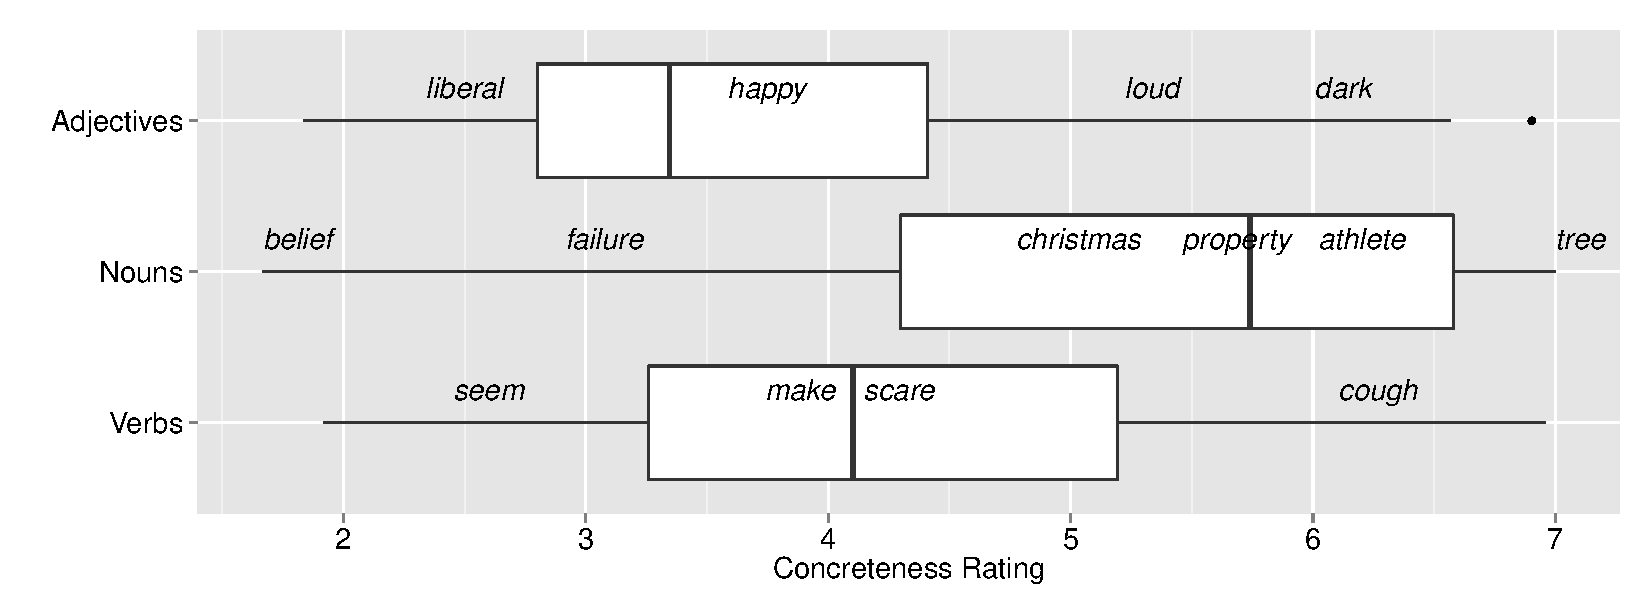
\includegraphics[width = \textwidth]{Chapter_3/Figure_1_CL}  \caption{Boxplots showing the interaction between concreteness and POS for concepts in USF. The white boxes range from the first to third quartiles and the central vertical line indicates the median.}\end{figure*}  

Unlike the POS distinction, concreteness  is generally considered to be a gradual phenomenon. One benefit of sampling pairs for SimLex-999 from the USF dataset is that most items have been rated according to concreteness on a scale of 1-7 by at least 10 human subjects. As Figure 1 demonstrates, concreteness (as the average over these ratings) interacts with POS on these concepts: nouns are on average more concrete than verbs which are more concrete than adjectives. However, there is also clear variation in concreteness within each POS category. We therefore aimed to select pairs for SimLex-999 that spanned the full abstract-concrete continuum within each POS category. 

After excluding any pairs that contained an item with no concreteness rating, for each potential SimLex-999 pair we considered both the concreteness of the first item and the additive difference in concreteness between the two items. This enabled us to stratify our sampling equally across four classes: (\( C_1\)) concrete first item (rating \(> 4\)) with below-median concreteness difference, (\( C_2\)) concrete first item (rating\( > 4\)), second item of lower concreteness and the difference being greater than the median, (\( C_3\)) abstract first item (rating \( \leq 4\)) with below-median concreteness difference, and (\( C_4\)) abstract first item (rating \(\leq 4\)) with the second item of greater concreteness and the difference being greater than the median. 

\paragraph{Final sampling} From the associated (USF) cohort of potential pairs we selected 600 noun pairs, 200 verb pairs and 100 adjective pairs, and from the unassociated (non-USF) cohort, we sampled 66 nouns pairs, 22 verb pairs and 11 adjective pairs. In both cases, the sampling was stratified such that, in each POS subset, each of the four concreteness classes \(C_1 - C_4\) was equally represented. 

\subsection{Question Design}

The annotator instructions for SimLex-999 are shown in Figure 2. We did not attempt to formalise the notion of similarity, but rather introduce it via the well-understood idea of synonymy, and in contrast to association. Even if a formal characterisation of similarity existed, the evidence in Section 2 suggests that the instructions would need separate cases to cover different concept types, increasing the difficulty of the rating task. Therefore we preferred to appeal to intuition on similarity, and to verify post-hoc that subjects were able to interpret and apply the informal characterization consistently for each concept type. 

\begin{figure*}[ht]  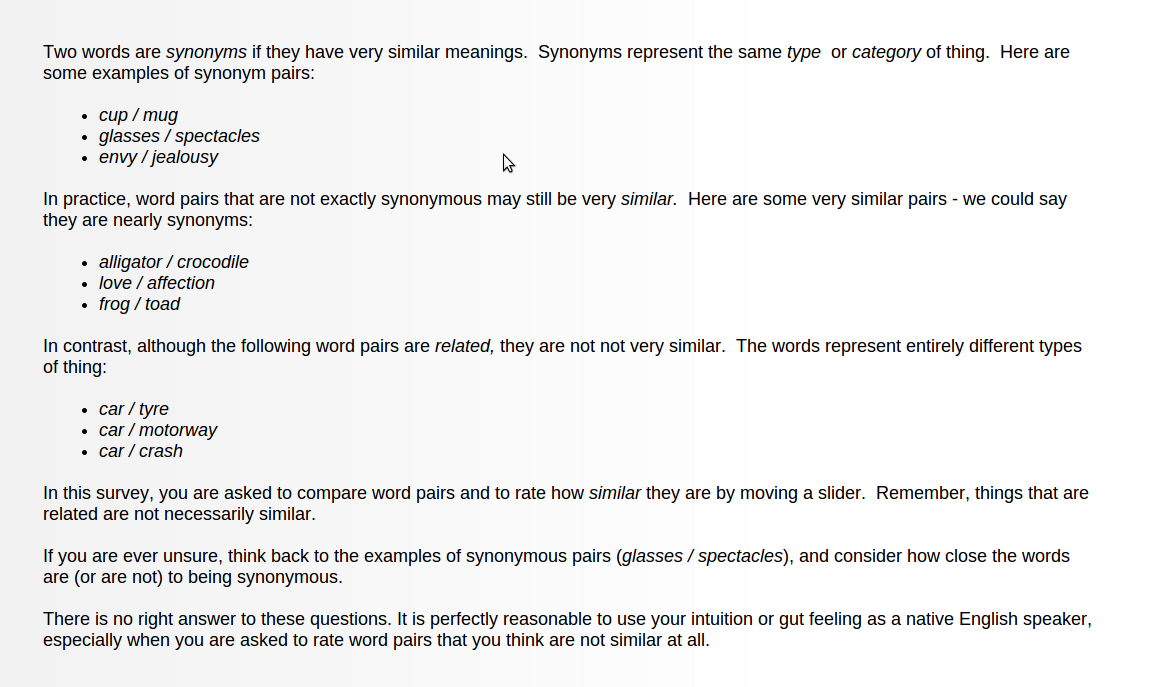
\includegraphics[width = \textwidth]{Chapter_3/screenshot1_CL}  \caption{Instructions for SimLex-999 annotators.}\end{figure*} 

Immediately following the instructions in Figure 2, participants were presented with two 'checkpoint' questions, one with abstract examples and one with concrete examples. In each case the participant was required to identify the \emph{most similar} pair from a set of three options, all of which were associated, but only one of which was clearly similar (e.g. [\emph{bread, butter}] [\emph{bread, toast}] [\emph{stale, bread}]). After this, the participants began rating pairs in groups of 6 or 7 pairs by moving a slider, as shown in Figure 3.

This group size was chosen because the (relative) rating a set of pairs implicitly requires pairwise comparisons between all pairs in that set. Therefore, larger groups would have significantly increased the cognitive load on the annotators. Another advantage of grouping was the clear break (submitting a set of ratings and moving to the next page) between the tasks of rating adjective, noun and verb pairs. For better inter-group calibration, from the second group onwards the last pair of the previous group became the first pair of the present group, and participants were asked to re-assign the rating previously attributed to the first pair before rating the remaining new items.  

\begin{wrapfigure}{r}{0.5\textwidth}

  \begin{center}

    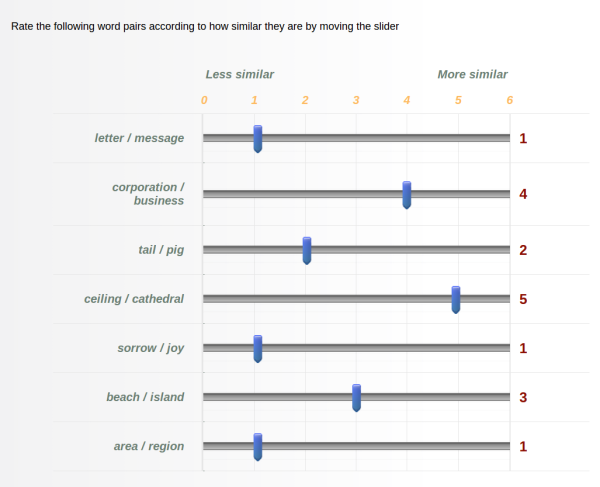
\includegraphics[width=0.5\textwidth]{Chapter_3/screenshot2_CL}

  \end{center}

  \caption{A group of noun pairs to be rated by moving the sliders. The rating slider was initially at position 0, and it was possible to attribute a rating of 0, although it was necessary to have actively moved the slider to that position to proceed to the next page.}

\end{wrapfigure}

%\begin{figure*}[ht]  \includegraphics[width = 0.5\textwidth]{screenshot2}  \caption{A group of noun pairs to be rated by moving the sliders. }\end{figure*}  


\vspace{2cm}
\subsection{Context-free rating}

As with MEN, WS-353 and RG, SimLex-999 consists of pairs of concept words together with a numerical rating. Thus, unlike in the small evaluation constructed by \cite{huang2012improving}, words are not rated in a phrasal or sentential context. Such meaning-in-context evaluations are motivated by a desire to disambiguate words that otherwise might be considered to have multiple senses.

We did not attempt to construct an evaluation based on meaning-in-context for several reasons. First, determining the set of senses for a given word, and then the set of contexts that represent those senses, introduces a high degree of subjectivity into the design process. Second, ensuring that a model has learned a high quality representation of a given concept would have required evaluating that concept in each of its given contexts, necessitating many more cases and a far greater annotation effort. Third, in the (infrequent) case that some concept \(c_1\) in an evaluation pair \((c_1,c_2)\) is genuinely (etymologically) polysemous, \( c_2 \) can provide sufficient context to disambiguate \(c_1\).\footnote{This is supported by the fact that the WordNet-based methods that perform best at modeling human ratings  model the similarity between concepts \( c_1 \) and \( c_2 \) as the minimum of all pairwise distances between the senses of \(c_1\) and the senses of \(c_2\) \cite{resnik1995using,pedersen2004wordnet}.} Finally, the POS grouping of pairs in the survey can also serve to disambiguate in the case that the conflicting senses of the polysemous concept are of differing POS category.

\subsection{Questionnaire structure}

Each participant was asked to rate 20 groups of pairs on a 0-6 scale of integers (non-integral ratings were not possible). Checkpoint multiple-choice questions were inserted at points between the 20 groups in order to ensure the participant had retained the correct notion of similarity. In addition to the checkpoint of three noun pairs presented before the first group (which contained noun pairs), checkpoint questions containing adjective pairs were inserted before the first adjective group and checkpoints of three verb pairs were inserted before the first verb group.     

From the 999 evaluation pairs, 14 noun pairs, 4 verb pairs and 2 adjective pairs were selected as a \emph{consistency set}. The dataset of pairs was then partitioned into 10 tranches, each consisting of 119 pairs, of which 20 were from the consistency set and the remaining 99 unique to that tranche. To reduce workload, each annotator was asked to rate the pairs in a single tranche only. The tranche itself was divided into 20 groups, with each group consisting of 7 pairs (with the exception of the last group of the 20, which had 6). Of these 7 pairs, the first pair was the last pair from the previous group, and the second pair was taken from the consistency set. The remaining pairs were unique to that particular group and tranche. The design enabled control for possible systematic differences between annotators and tranches, which could be detected by variation on the consistency set. 

\subsection{Participants}

500 residents of the USA were recruited from Mechanical Turk, each with at least 95\% approval rate for work on the web service. Each participant was required to check a box confirming that he or she was a native speaker of English and warned that work would be rejected if the pattern of responses indicated otherwise. The participants were distributed evenly to rate pairs in one of the ten question tranches, so that each pair was rated by approximately 50 subjects. Participants took between 8 and 21 minutes to rate the 119 pairs across the 20 groups, together with the checkpoint questions. 

\subsection{Post-processing}

In order to correct for systematic differences in the overall calibration of the rating scale between respondents, we measured the average (mean) response of each rater on the consistency set. For 32 respondents, the absolute difference between this average and the mean of all such averages was greater than one (though never greater than two); i.e. 32 respondents demonstrated a clear tendency to rate pairs as either more or less similar than the overall rater population. To correct for this bias, we increased (or decreased) the rating of such respondents for each pair by one, except in cases where they had given the maximum rating, six (or minimum rating, zero). This adjustment, which ensured that the average response of each participant was within one of the mean of all respondents on the consistency set, resulted in a small increase to the inter-rater agreement on the dataset as a whole.     

After controlling for systematic calibration differences, we imposed three conditions for the responses of a rater to be included in the final data collation.  First, the average pairwise Spearman correlation of responses with all other responses for a participant could not be more than one standard deviation below the mean of all such averages. Second, the increase in inter-rater agreement when a rater was excluded from the analysis needed to be smaller than at least 50 other raters (i.e. 10\% of raters were excluded on this criterion). Third, we excluded the 6 participants who got one or more of the checkpoint questions wrong. A total of 99 participants were excluded based on one or more of these conditions, but no more than 16 from any one tranche (so that each pair in the final dataset was rated by a minimum of 36 raters). Finally, we computed average (mean) scores for each pair, and transformed all scores linearly from the interval \([0,6]\) to the interval \([0,10]\).

\section{Analysis of Dataset}

In this section we analyse the responses of the SimLex-999 annotators and the resulting ratings. First, by considering inter-annotator agreement we examine the consistency with which annotators were able to apply the characterization of similarity outlined in the instructions to the range of concept types in SimLex-999. Second, we verify that a valid notion of similarity was understood by the annotators, in that they were able to accurately separate similarity from association. 

\subsection{Inter-annotator agreement}

\begin{figure*}[ht]  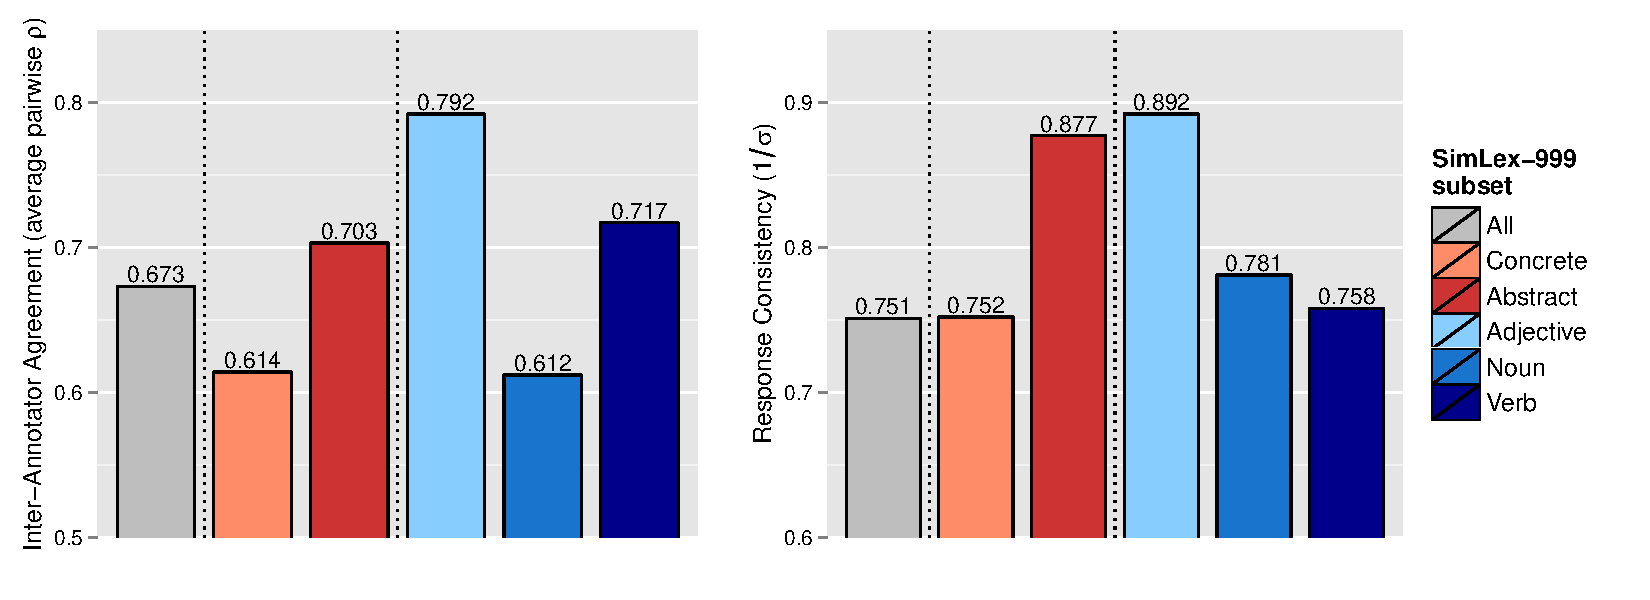
\includegraphics[width = \textwidth]{Chapter_3/Figure_1A_CL}  \caption{{\bf Left:} Inter-annotator agreement, measured by average pairwise Spearman \(\rho\) correlation, for ratings of concept types in SimLex-999. {\bf Right:} Response consistency, reflecting the standard deviation of annotator ratings for each pair, averaged over all pairs in the concept category.}\end{figure*}  

As in previous annotation or data collection for computational semantics \cite{pado2007flexible,reisinger2010mixture,silberer2014learning} we computed the inter-rater agreement as the average of pairwise Spearman \(\rho\) correlations between the ratings of all respondents. Overall agreement was \(\rho=0.67\). This compares favourably with the agreement on WS-353 (\(\rho=0.61\) using the same method). The design of the MEN rating system precludes a conventional calculation of inter-rater agreement \cite{bruni2012distributional2}. However, two of the creators of MEN who independently rated the dataset achieved an agreement of \(\rho=0.68\).\footnote{Reported at http://clic.cimec.unitn.it/~elia.bruni/MEN. It is reasonable to assume that actual agreement on MEN may be somewhat lower than 0.68 given the small sample size and the expertise of the raters.} 

The SimLex-999 inter-rater agreement suggests that participants were able to understand the (single) characterization of similarity presented in the instructions and to apply it to concepts of various types consistently. This conclusion was supported by inspection of the brief feedback offered by the majority of annotators in a final text field in the questionnaire: 78\% expressed sentiment that the test was clear, easy to complete or some similar sentiment.

Interestingly, as shown in Figure 4 (left), agreement was not uniform across the concept types. Contrary to what might be expected given established concreteness effects \cite{paivio1991dual}, we observed not only higher inter-rater agreement but also less per-pair variability for abstract rather than concrete concepts\footnote{Per-pair variability was measured by calculating the standard deviation of responses for each pair, and averaging these scores across the pairs of each concept type.}. 

Strikingly, the highest inter-rater consistency and lowest per-pair variation (defined as the inverse of the standard deviation of all ratings for that pair) was observed on adjective pairs. While we are unsure exactly what drives this effect, a possible cause is that many pairs of adjectives in SimLex-999 cohabit a single salient, one-dimensional scale (\emph{freezing > cold > warm > hot}). This may be a consequence of the fact that many pairs in SimLex-999 were selected (from USF) to have a degree of association. On inspection, pairs of nouns and verbs in SimLex-999 do not appear to occupy scales in the same way, possibly since concepts of these POS categories come to be associated via a more diverse range of relations. It seems plausible that humans are able to estimate the similarity of scale-based concepts more consistently than pairs of concepts related in a less uni-dimensional fashion. 

Regardless of cause, however, the high agreement on adjectives is a satisfactory property of SimLex-999. Adjectives exhibit various aspects of lexical semantics that have proved challenging for computational models, including antonymy, polarity \cite{williams2009predicting} and sentiment \cite{wiebe2000learning}. To approach the high level of human confidence on the adjective pairs in SimLex-999, it may be necessary to focus particularly on developing automatic ways to capture these phenomena. 

\subsection{Response validity: Similarity not association}	



Inspection of the SimLex-999 ratings indicated that pairs were indeed evaluated according to similarity rather than association. Table 2 includes examples that demonstrate a clear dissociation between the two semantic relations. 



 \begin{table}[t]\begin{center}\begin{tabular}{l|l|c|r|r|r|r}





C1 & C2 & POS & USF* & USF rank (of 999) & SimLex & SimLex rank (of 999) \\



\hline \emph{dirty} & \emph{narrow} & A & 0.00 & 999 & 0.30 & 996 \\



\emph{student} & \emph{pupil} & N & 6.80 & 12 & 9.40 & 12 \\

\emph{win} & \emph{dominate} & V & 0.41 & 364 & 5.68 & 361 \\



\hdashline \emph{smart} & \emph{dumb} & A & 2.10 & 92 & 0.60 & 947 \\

\emph{attention} & \emph{awareness} & N &  0.10 & 895 & 8.73 & 58 \\

\emph{leave} & \emph{enter} & V & 2.16 & 89 & 1.38 & 841 \\
\end{tabular}
\end{center}\caption{\label{font-table} {\bf Top:  Similarity aligns with association} Pairs with a small difference in rank between USF (association) and SimLex-999 (similarity) scores for each POS category. {\bf Bottom: Similarity contrasts with association} Pairs with a high difference in rank for each POS category. *Note that the distribution of USF association scores on the interval [0,10] is highly skewed towards the lower bound in both SimLex-999 and the USF dataset as a whole.}\end{table}

\begin{figure*}[ht]  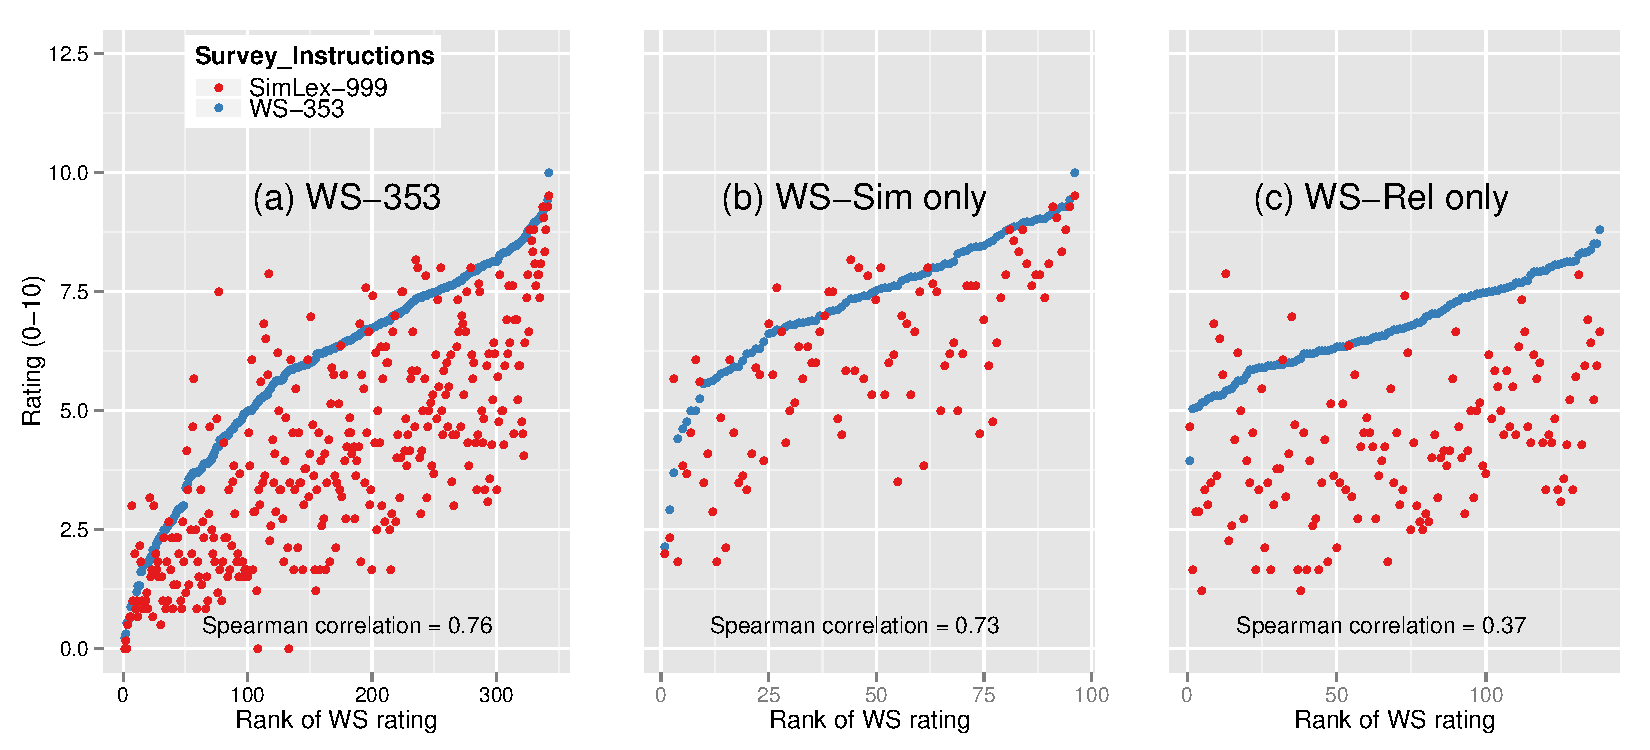
\includegraphics[width =\textwidth]{Chapter_3/Figure_6_CL} \caption{{\bf(a)} Pairs rated by WS-353 annotators (blue points, ranked by rating) and the corresponding rating of annotators following the SimLex-999 instructions (red points). {\bf(b-c)} The same analysis, restricted to pairs in the WS-Sim or WS-Rel subsets of WS-353.}\end{figure*}  



To verify this effect quantitatively, we recruited 100 additional participants to rate the WS-353 pairs, but following the SimLex-999 instructions and question format. As shown in Fig 5(a), there were clear differences between these new ratings and the original WS-353 ratings. In particular, a high proportion of pairs was given a lower rating by subjects following the SimLex-999 instructions than those following the WS-353 guidelines: The mean SimLex rating was 4.07 compared with 5.91 for WS-353. 



This was consistent with our expectations that pairs of associated but dissimilar concepts would receive lower ratings based on the SimLex-999 than on the WS-353 instructions while pairs that were both associated and similar would receive similar ratings in both cases. To confirm this, we compared the WS-353 and SimLex-999-based ratings on the subsets WS-Rel and WS-Sim, which were hand-sorted by \cite{agirre2009study} to include pairs connected by association (and not similarity) and those connected by similarity (but possibly also association) respectively.  



As shown in Figure 5(b-c), the correlation between the SimLex-999-based and WS-353 ratings was notably higher (\(\rho=0.73\)) on the WS-Sim subset than the WS-Rel subset (\(\rho=0.38\)). Specifically, the tendency of subjects following the SimLex-999 instructions to assign lower ratings than those following the WS-353 instructions was far more pronounced for pairs in WS-Sim (Figure 5(b)) than for those in WS-Rel (5(c)). This observation suggest that the associated but dissimilar pairs in WS-353 were an important driver of the overall lower mean for SimLex-999-based ratings, and thus provide strong evidence that the SimLex-999 instructions do indeed enable subjects to distinguish similarity from association effectively. 


\subsection{Finer-grained Semantic Relations}

We have established the validity of similarity as a notion understood by human raters and distinct from association. However, much theoretical semantics focuses on relations between words or concepts that are finer-grained than similarity and association. These include \emph{meronymy} (a part to its whole, e.g. \emph{blade - knife}), \emph{hypernymy} (a category concept to a member of that category, e.g. \emph{animal - dog}) and \emph{cohyponymy} (two members of the same implicit category, e.g. the pair of animals \emph{dog - cat}) \cite{cruse1986lexical}. Beyond theoretical interest, these relations can have practical relevance. For instance, hypernymy can form the basis of semantic entailment and therefore textual inference: the proposition \emph{a cat is on the table} entails that \emph{an animal is on the table} precisely because of the hypernymy relation from animal to cat. 

We chose not to make these finer-grained relations the basis of our evaluation for several reasons. At present, detecting relations such as hypernymy using distributional methods is challenging, even when supported by supervised classifiers with access to labelled pairs \cite{levy2015supervised}. Such a designation can seem to require specific world-knowledge (is a \emph{snale} a \emph{reptile}?), can be gradual, as evidenced by typicality effects \cite{rosch1976structural}, or simply highly subjective. Moreover, a fine-grained relation \(R\) will only be attested (to any degree) between a small subset of all possible word pairs, whereas similarity can in theory be quantified for any two words chosen at random. We thus considered a focus on fine-grained semantic relations to be less appropriate for a general-purpose evaluation of representation quality.  

Nevertheless, post-hoc analysis of the SimLex annotator responses and fine-grained relation classes, as defined by lexicographers, yields further interesting insights into the nature of both similarity and association. Of the 999 word pairs in SimLex, 382 are also connected by one of the common finer-grained semantic relations in WordNet. For each of these relations, Figure 6 shows the average similarity rating and average USF free association score for all pairs that exhibit that relation. 

In cases where a relationship of hypernymy/hyponymy exists between the words in a pair (not necessarily immediate - \(1\_hypernym, 2\_hypernym\) etc.) similarity and association coincide. Hyper/hyponym pairs that are separated by fewer levels in the WordNet hierarchy are both more strongly associated and rated as more similar. However, there are also interesting discrepancies between similarity and association. Unsurprisingly, pairs that are classed as synonyms in WordNet (i.e. having at least one sense in some common synset) are rated as more similar than pairs of any other relation type by SimLex annotators. In contrast, antonyms are the most strongly-associated word pairs among these finer-grained relations. Further, pairs consisting of a meronym and holonym (part and whole) are comparatively strongly associated but not judged to be similar. 

The analysis also highlights a case that can be particularly problematic when rating similarity;  cohyponyms, or members of the same salient category (such as \emph{knife} and \emph{fork}). We gave no specific guidelines for how to rate such pairs in the SimLex annotator instructions, and whether they are considered similar or not seems to be a matter of perspective. On one hand, their membership of a common category could make them appear similar, particularly if the category is relatively specific. On the other hand, in the case of \emph{knife} and \emph{fork}, for instance, the underlying category \emph{cultery} might provide a backdrop against which the differences of distinct members become particularly salient. 

\begin{figure}[ht]  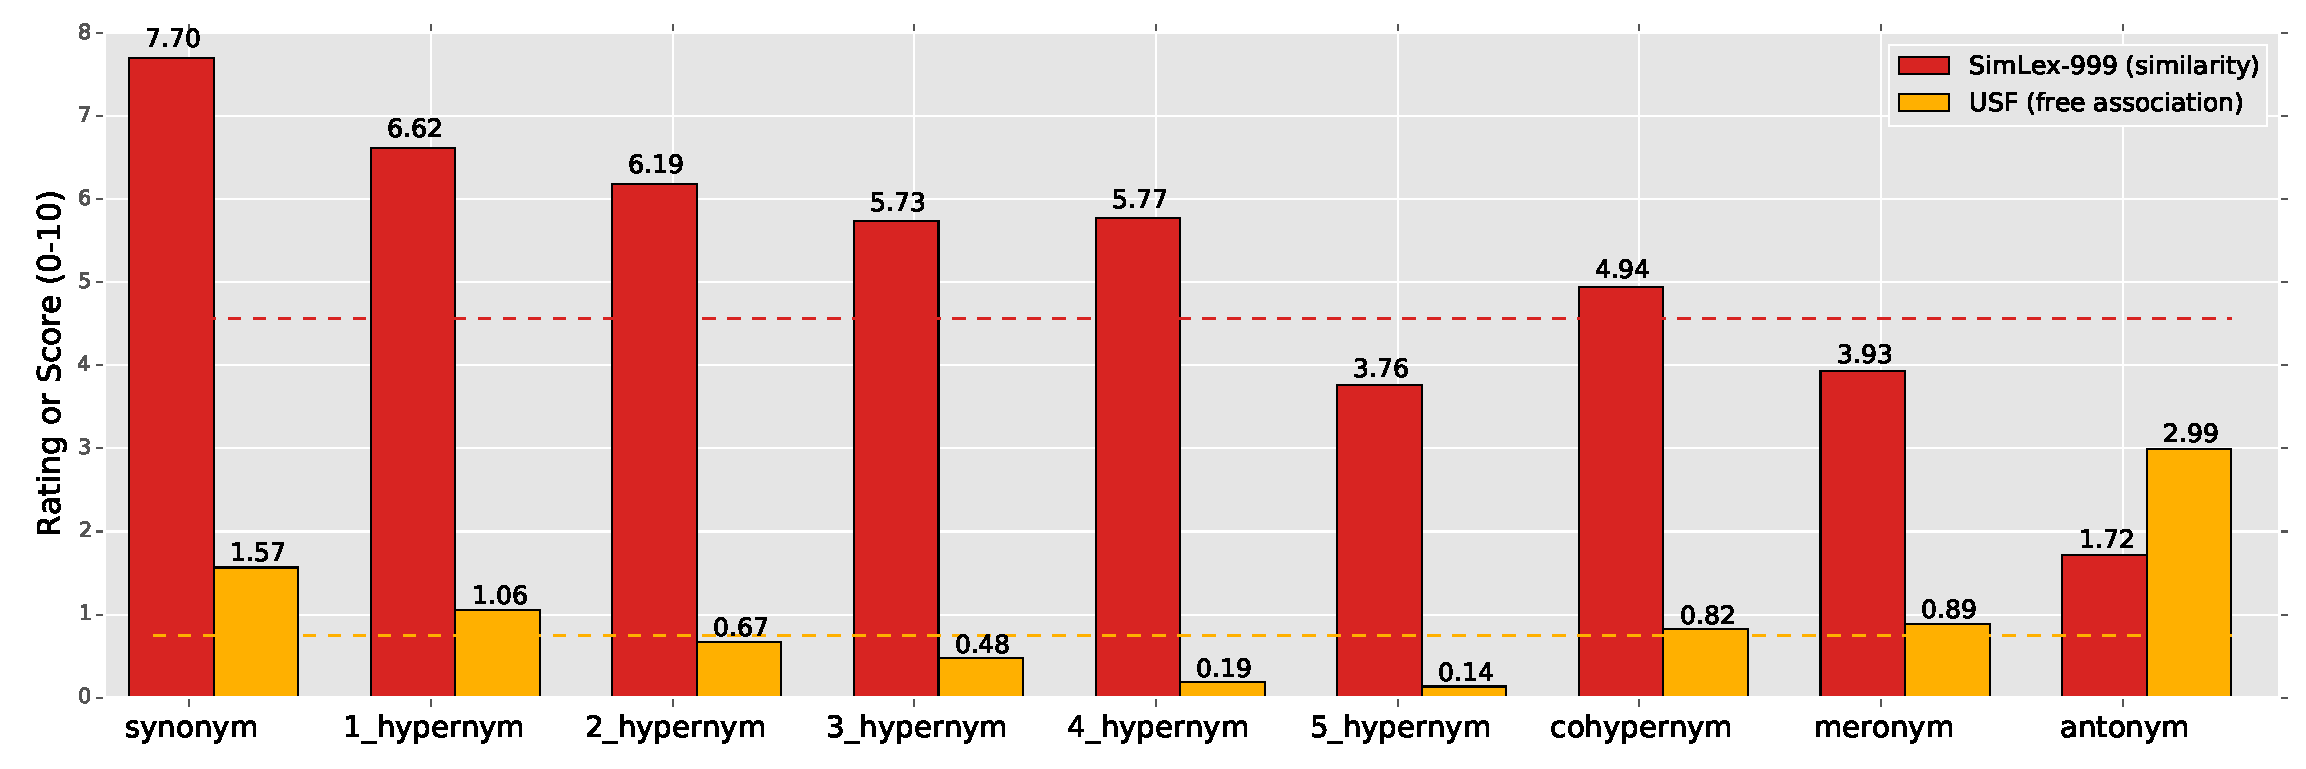
\includegraphics[width =\textwidth]{Chapter_3/simlex_relations_CL}  \caption{Average SimLex and USF free association scores across pairs representing different fine-grained semantic relations. All relations were extracted from WordNet. \(n\_hypernym\) refers to a direct hypernymy path of length \(n\). Note that the average SimLex rating across all 999 word pairs (dashed red line) is much higher than the average USF rating (dashed golden line) because of differences in the rating procedure. The more interesting differences concern the relative strength of similarity vs. association across the different relation types.}\end{figure}  

\section{Evaluating Models with SimLex-999}

In this section, we demonstrate the applicability of SimLex-999 by analysing the performance of various distributional semantic models in estimating the new ratings. The models were selected to cover the main classes of representation learning architectures \cite{baroni2014don}: Vector space co-occurrence (counting) models and neural language models (NLM)s \cite{Bengio2003lm}. We first show that SimLex-999 is notably more difficult for state-of-the-art models to estimate than existing gold standards. We then conduct more focused analyses on the various concept subsets defined in SimLex-999, exploring possible causes for the comparatively low performance of current models and, in turn, demonstrating how SimLex-999 can be applied to investigate such questions.    

\subsection{Semantic models}

\paragraph{\bf Collobert \& Weston}

\cite{collobert2008unified} apply the architecture of an NLM to learn a word representations \(v_w\) for each word \(w\) in some corpus vocabulary \( V\). Each sentence \( s\) in the input text is represented by a matrix containing the vector representations of the words in \(s\) in order. The model then computes output scores \(f(s) \) and \(f(s^w) \), where \(s^w\) denotes an `incorrect' sentence created from \(s\) by replacing its last word with some other word \( w\) from \(V\). Training involves updating the parameters of the function \(f\) and the entries of the vector representations \(v_w\) such that  \(f(s)\) is larger than \(f(s^w) \) for any \(w\) in \(V\), other than the correct final word of \(s\). This corresponds to minimising the sum of the following sentence objectives \( C_s\) over all sentences in the input corpus, which is achieved via (mini-batch) stochastic gradient descent:

\[ C_{s}  = \sum_{w \in V} max(0,1-f(s) + f(s^w)). \]

The relatively low-dimension, dense (vector) representations learned by this model and the other NLMs introduced in this section are sometimes referred to as \emph{embeddings} \cite{turian2010word}. \cite{collobert2008unified} train their models on 852 million words of text from a 2007 dump of Wikipedia and the RCV1 Corpus \cite{lewis2004rcv1} and use their embeddings to achieve state-of-the-art results on a variety of NLP tasks. We downloaded the embeddings directly from the authors' webpage.\footnote{http://ml.nec-labs.com/senna/}

 \paragraph{\bf Huang et al.}

\cite{huang2012improving} present a NLM that learns word embeddings to maximise the likelihood of predicting the last word in a sentence \(s\) based on (i) the previous words in that sentence (local context - as with \cite{collobert2008unified}) and (ii) the document \( d\) in which that word occurs (global context). As with \cite{collobert2008unified}, the model represents input sentences as a matrix of word embeddings. In addition, it represents documents in the input corpus as single-vector averages over all word embeddings in that document. It can then compute scores \(g(s,d )\) and \(g(s^w, d) \), where as before \(s^w\) is a sentence with an `incorrect' randomly-selected last word. Training is again by stochastic gradient descent, and corresponds to minimising the sum of the sentence objectives \(C_{s,d} \) over all of the sentences in the corpus:

\[ C_{s,d}  = \sum_{w \in V} max(0,1-g(s,d) + g(s^w,d)). \]

The combination of local and global contexts in the objective encourages the final word embeddings to reflect aspects of both the meaning of nearby words and of the documents in which those words appear. When learning from 990m words of wikipedia text, Huang et al. report a Spearman correlation of \(\rho = 71.3\) between the cosine similarity of their model embeddings and the WS-353 scores, which constitutes state-of-the-art performance for a NLM model on that dataset. We downloaded these embeddings from the authors' webpage.\footnote{\url{www.socher.org/index.php/Main/ImprovingWordRepresentationsViaGlobalContextAndMultipleWordPrototypes}.}

\paragraph{\bf Mikolov et al.}

\cite{mikolov2013efficient} present an architecture that learns word embeddings similar to those of standard NLMs but with no non-linear hidden layer (resulting in a simpler scoring function). This enables faster representation learning for large vocabularies. Despite this simplification, the embeddings achieve state-of-the-art performance on several semantic tasks including sentence completion and analogy modelling \cite{mikolov2013efficient,mikolov2013distributed}.   

For each word type \(w\) in the vocabulary \(V\), the model learns both a `target-embedding' \( r_{w} \in \mathbb{R}^d\) and a `context-embedding' \(\hat{r}_{w} \in \mathbb{R}^d\) such that, given a target word, its ability to predict nearby context words is maximised. The probability of seeing context word \(c\) given target \(w\) is defined as:  

\[p(c|w)  = \frac{\me^{\hat{r}_{c} \cdot r_{w}}}{\sum_{v \in V} \me^{\hat{r}_v\cdot r_{w}}}.\]

The model learns from a set of (target-word, context-word) pairs, extracted from a corpus of sentences as follows. In a given sentence \(s\) (of length \(N\)), for each position \( n \leq N\), each word \(w_n\) is treated in turn as a target word. An integer \( {t(n)} \) is then sampled from a uniform distribution on \( \{1, \dots k \} \), where \(k > 0\) is a predefined maximum context-window parameter. The pair tokens \( \{(w_n, w_{n+j}): -{t(n)}\leq j \leq {t(n)}, w_i \in s \}\) are then appended to the training data. Thus, target/context training pairs are such that (i) only words within a \(k\)-window of the target are selected as context words for that target, and (ii) words closer to the target are more likely to be selected than those further away.

The training objective is then to maximise the log probability \( T\), defined below, across of all such examples from \(s\), and then across all sentences in the corpus. This is achieved by stochastic gradient descent. 

\[ T = \frac{1}{N} \sum_{n=1}^{N} \sum_{-{t(n)}\leq j \leq {t(n)}, j\neq 0} log(  p(w_{n+j}|w_{n}) ) \]

As with other NLMs, Mikolov et al.'s model captures conceptual semantics by exploiting the fact that words appearing in similar linguistic contexts are likely to have similar meanings. Informally, the model adjusts its embeddings to increase the probability of observing the training corpus. Since this probability increases with \(p(c|w)\), and \(p(c|w)\) increases with the dot product \( \hat{r}_c\cdot r_{w} \), the updates have the effect of moving each target-embedding incrementally `closer' to the context-embeddings of its collocates. In the target-embedding space, this results in embeddings of concept words that regularly occur in similar contexts moving closer together.  

We use the author's Word2vec software in order to train their model and use the target embeddings in our evaluations. We experimented with embeddings of dimension 100, 200, 300, 400 and 500 and found that 200 gave the best performance on both WS-353 and SimLex-999. 

\paragraph{\bf Vector Space Model (VSM)}

As an alternative to NLMs, we constructed a vector space model following the guidelines for optimal performance outlined by \cite{kiela2014systematic}. After extracting the 2000 most frequent word tokens in the corpus that are not in a common list of stopwords\footnote{Taken from the Python Natural Language Toolkit \cite{bird2006nltk}.} as features, we populated a matrix of co-occurrence counts with a row for each of the concepts in some pair in our evaluation sets, and a column for each of the features. Co-occurrence was counted within a specified window size, although never across a sentence boundary. This resulting matrix was then weighted according to Pointwise Mutual Information (PMI) \cite{recchia2009more}. The rows of the resulting matrix constitute the vector representations of the concepts.   

\paragraph{\bf SVD} As proposed initially in \cite{landauer1997solution}, we also experimented with models in which Singular Value Decomposition (SVD) \cite{golub1970singular} is applied to the PMI-weighted VSM matrix, reducing the dimension of each concept representation to 300 (which yielded best results after experimenting, as before, with 100-500 dimension vectors). 

\vspace{1\baselineskip}

\noindent 
For each model described in this section, we calculate similarity as the cosine similarity between the (vector) representations learned by that model. 

\subsection{Results}

In experimenting with different models on SimLex-999, we aimed to answer the following questions: (i) How well do the established models perform on SimLex-999 versus on existing gold standards? (ii) Are any observed differences caused by the potential of different models to measure similarity vs. association? (iii) Are there interesting differences in ability of models to capture similarity between adjectives vs nouns vs verbs? (iv) In this case, are the observed differences driven by concreteness, and its interaction with POS, or are other factors also relevant?

\paragraph{\bf Overall performance on SimLex-999}

\begin{figure*}[ht]  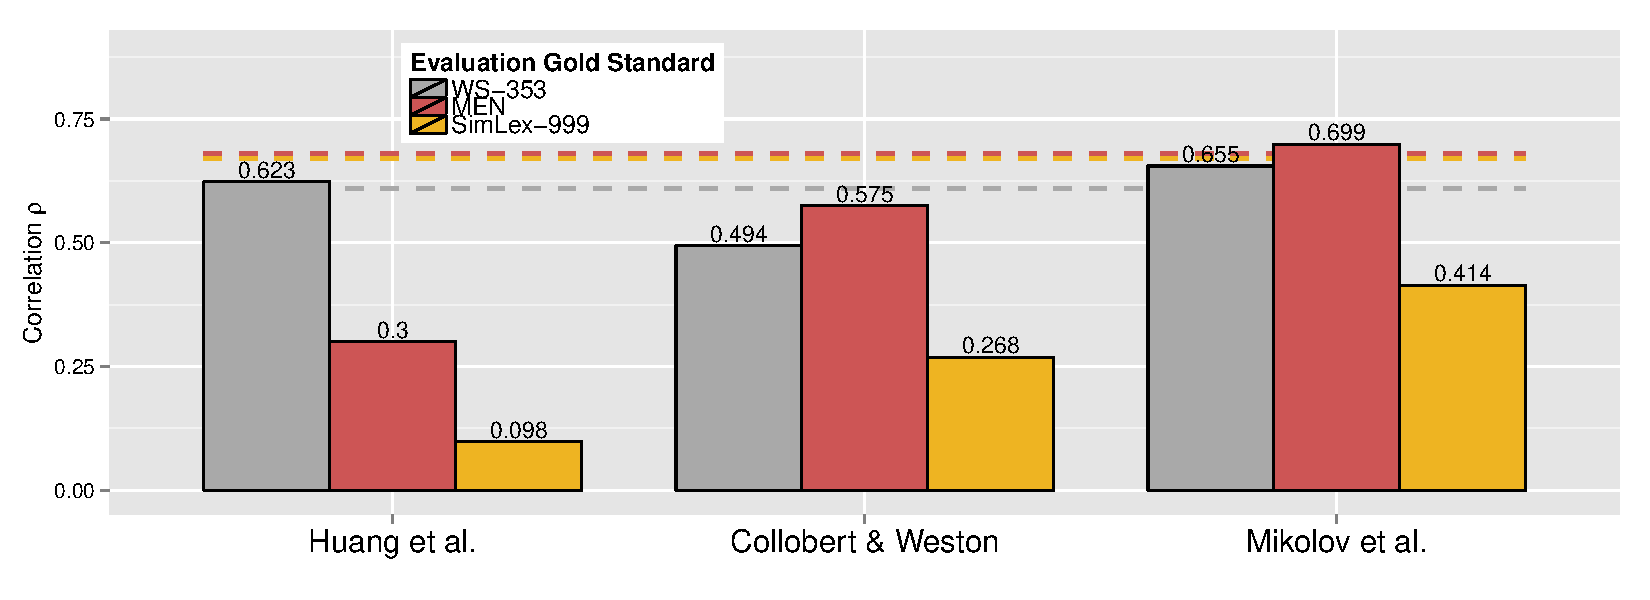
\includegraphics[width = \textwidth, height=5cm]{Chapter_3/Figure_2A_CL} \caption{Performance of NLMs on WS-353, MEN and SimLex-999. All models are trained on Wikipedia; note that as Wikipedia is constantly growing, the \protect\cite{mikolov2013efficient} model exploited slightly more training data ($\approx$1000m tokens) than the \protect\cite{huang2012improving} model ($\approx$990m), which in turn exploited more than the \protect\cite{collobert2008unified} model ($\approx$852m). Dashed horizontal lines indicate the level of inter-annotator agreement for the three datasets.}\end{figure*}

\begin{figure*}[ht]  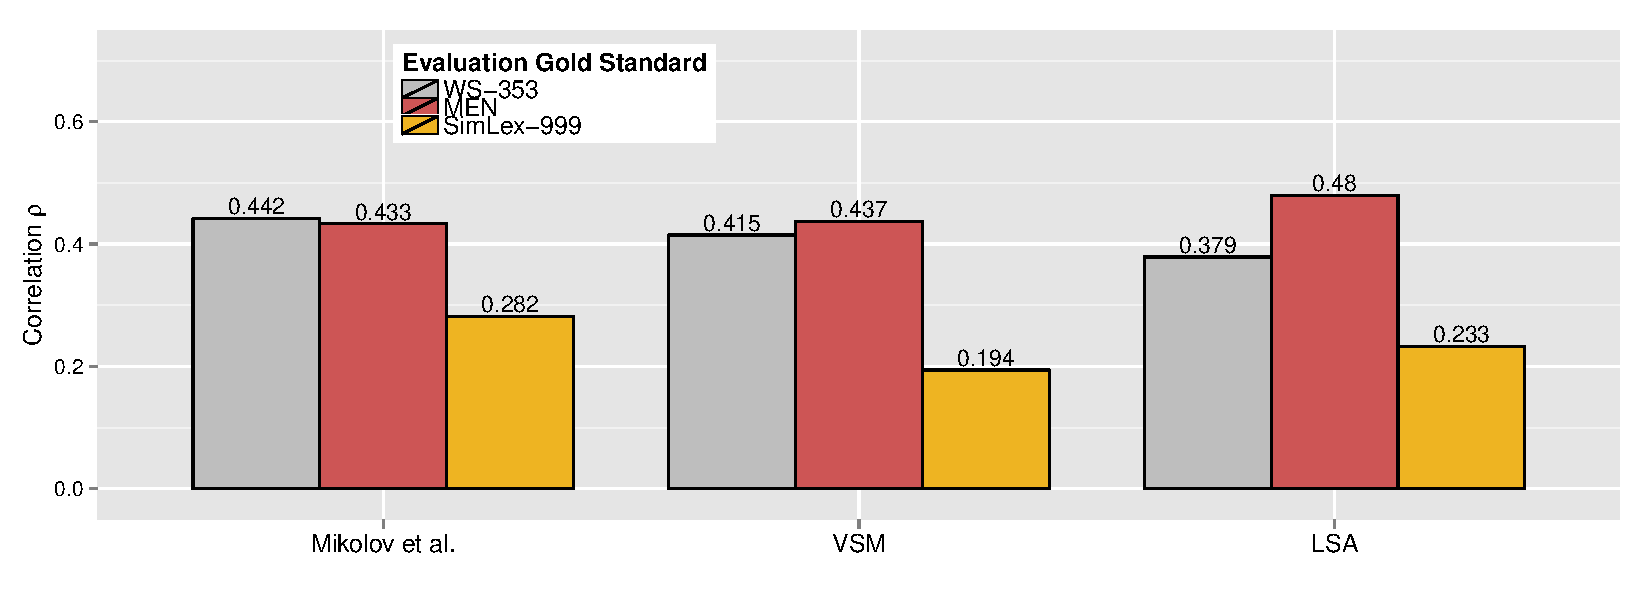
\includegraphics[width = \textwidth,height=5cm]{Chapter_3/Figure_2B_CL}  \caption{Comparison between the leading NLM, \emph{Mikolov et al.}, the vector space model, \emph{VSM}, and the \emph{SVD} model. All models were trained on the $\approx$150m word RCV1 Corpus \protect\cite{lewis2004rcv1}.}\end{figure*}

Figure 7 shows the performance of the NLMs on SimLex-999 versus on comparable datasets, measured by Spearman's \(\rho\) correlation. All models estimate the ratings of MEN and WS-353 more accurately than SimLex-999. The \cite{huang2012improving} model performs well on WS-353,\footnote{This score, based on embeddings downloaded from the authors' webpage, is notably lower than the score reported in \cite{huang2012improving} mentioned in Section 5.1.} but is not very robust to changes in evaluation gold standard, and performs worst of all the models on SimLex-999. Given the focus of the WS-353 ratings, it is tempting to explain this by concluding that the global context objective leads the \cite{huang2012improving} model to focus on association rather than similarity. However, the true explanation may be less simple, since the \cite{huang2012improving} model performs weakly on the association-based MEN dataset. The \cite{collobert2008unified} model is more robust across WS-353 and MEN, but still does not match the performance of the \cite{mikolov2013efficient} model on SimLex-999. 

Figure 8 compares the best performing NLM model \cite{mikolov2013efficient} with the VSM and SVD models.\footnote{We conduct this comparison on the smaller RCV1 Corpus \cite{lewis2004rcv1} because training the VSM and SVD models is comparatively slow.}  In contrast to recent results that emphasise the superiority of NLMs over alternatives \cite{baroni2014don}, we observed no clear advantage for the NLM over the VSM or SVD when considering the association-based gold standards WS-353 and MEN together. While the NLM is the strongest performer on WS-353, SVD is the strongest performer on MEN. However, the NLM model performs notably better than the alternatives at modelling similarity, as measured by SimLex-999. 

Comparing all models in Figures 7 and 8 suggests that SimLex-999 is notably more challenging to model than the alternative datasets, with correlation scores ranging from 0.098 to 0.414. Thus, even when state-of-the-art models are trained for several days on massive text corpora, \footnote{Training times reported by \cite{huang2012improving} and for \cite{collobert2008unified} at \url{http://ronan.collobert.com/senna/}.} their performance on SimLex-999 is well below the inter-annotator agreement (Figure 7). This suggests that there is ample scope for SimLex-999 to guide the development of improved models. 

\paragraph{\bf Modeling similarity vs. association}

The comparatively low performance of NLM, VSM and SVD models on SimLex-999 compared with MEN and WS-353 is consistent with our hypothesis that modelling similarity is more difficult than modelling association. Indeed, given that many strongly-associated but dissimilar pairs, such as [\emph{coffee, cup}], are likely to have high co-occurrence in the training data, and that all models infer connections between concepts from linguistic co-occurrence in some form or another, it seems plausible that models may overestimate the similarity of such pairs because they are `distracted' by association.

To test this hypothesis more precisely, we compared the performance of models on the whole of SimLex-999 versus its 333 most associated pairs (according to the USF free association scores). Importantly, pairs in this strongly-associated subset still span the full range of possible similarity scores (min similarity = 0.23 [\emph{shrink, grow}], max similarity = 9.80 [\emph{vanish, disappear}]).     

As shown in Figure 9, all models performed worse when the evaluation was restricted to pairs of strongly-associated concepts, which was consistent with our hypothesis. The \cite{collobert2008unified} model was better than the \cite{huang2012improving} model at estimating similarity in the face of high association. This not entirely surprising given the global-context objective in the latter model, which may have encouraged more association-based connections between concepts. The Mikolov et al. model, however, performed notably better than both other NLMs. Moreover, this superiority is proportionally greater when evaluating on the most associated pairs only (as indicated by the difference between the red and grey bars), suggesting that the improvement is driven at least in part by an increased ability to `distinguish' similarity from association. 

\begin{figure*}[]  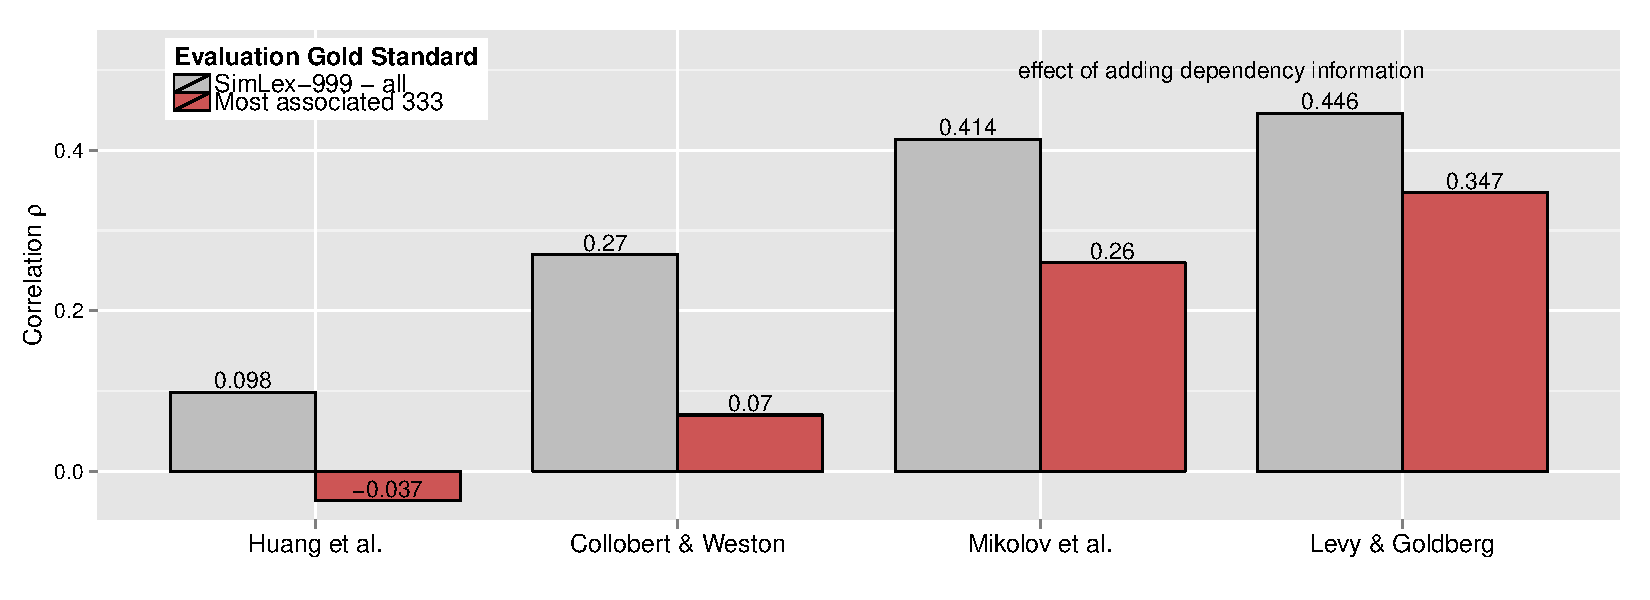
\includegraphics[width = \textwidth,height=5cm]{Chapter_3/Figure_3A_CL}  \caption{The ability of NLMs to model the similarity of highly-associated concepts versus concepts in general. The two models on the right hand side also demonstrate the effect of training an NLM (the \protect\cite{mikolov2013efficient} model) on running-text (\emph{Mikolov et al.}) vs. on dependency-based input (\emph{Levy \& Goldberg}).}\end{figure*}

\begin{figure*}[]  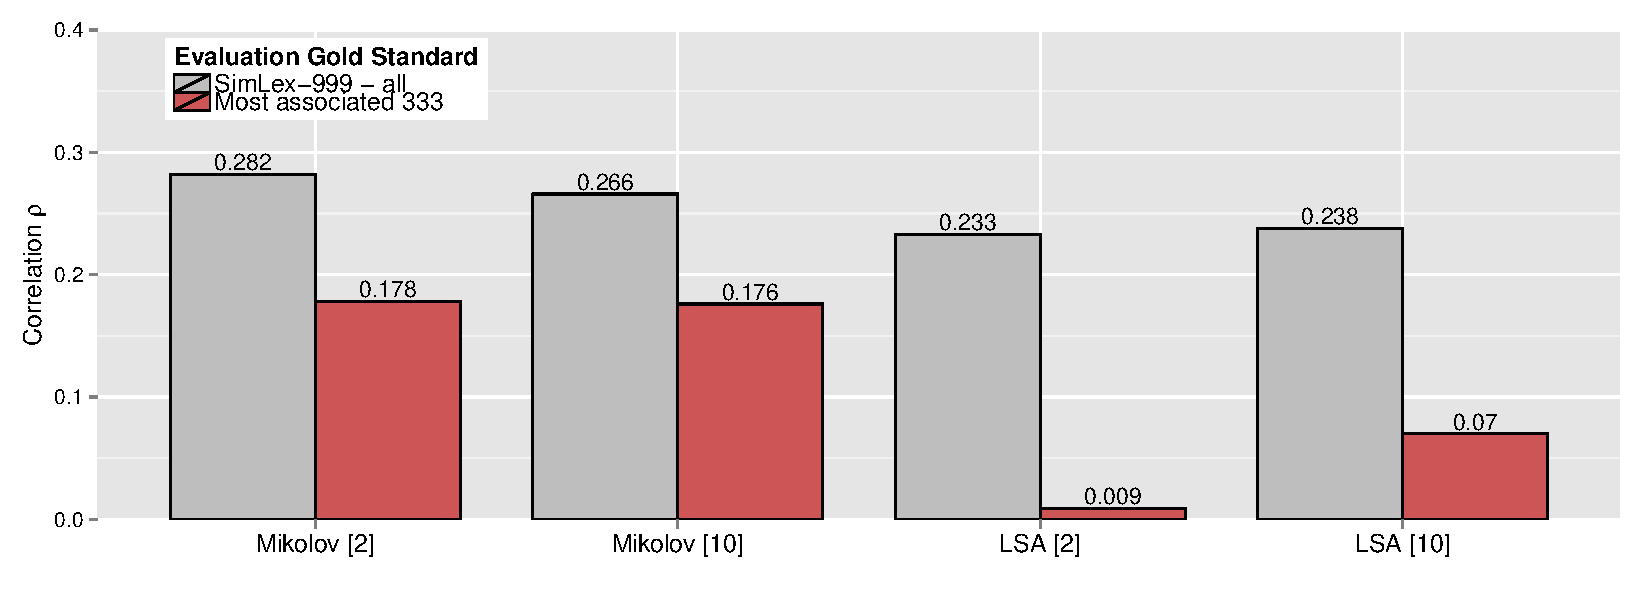
\includegraphics[width = \textwidth,height=5cm]{Chapter_3/Figure_3B_CL}  \caption{The effect of different window sizes (indicated in square brackets [ ]) on NLM and SVD models. }\end{figure*}

To understand better how the architecture of models captures information pertinent to similarity modelling, we performed two additional experiments using SimLex-999. These comparisons were also motivated by the hypotheses, made in previous studies and outlined in Section 2.1.2, that both dependency-informed input and smaller context windows encourage models to capture similarity rather than association. 

We tested the first hypothesis using the embeddings of \cite{levy2014dependency}, whose model extends the \cite{mikolov2013efficient} model so that target-context training instances are extracted based on dependency-parsed rather than simple running text. As illustrated in Figure 9, the dependency-based embeddings outperform the original (running text) embeddings trained on the same corpus. Moreover, the comparatively large increase in the red bar compared to the grey bar suggests that an important part of the improvement of the dependency-based model derives from a greater ability to discern similarity from association. 

Our comparisons provided less support for the second (window size) hypothesis. As shown in Figure 10, there is a negligible improvement in the performance of the \cite{} model when the window size is reduced from 10 to 2. However, for the SVD model we observed the converse. The SVD model with window size 10 slightly outperforms the SVD model with window 2, and this improvement is quite pronounced on the most associated pairs in SimLex-999. 

\begin{figure*}[]  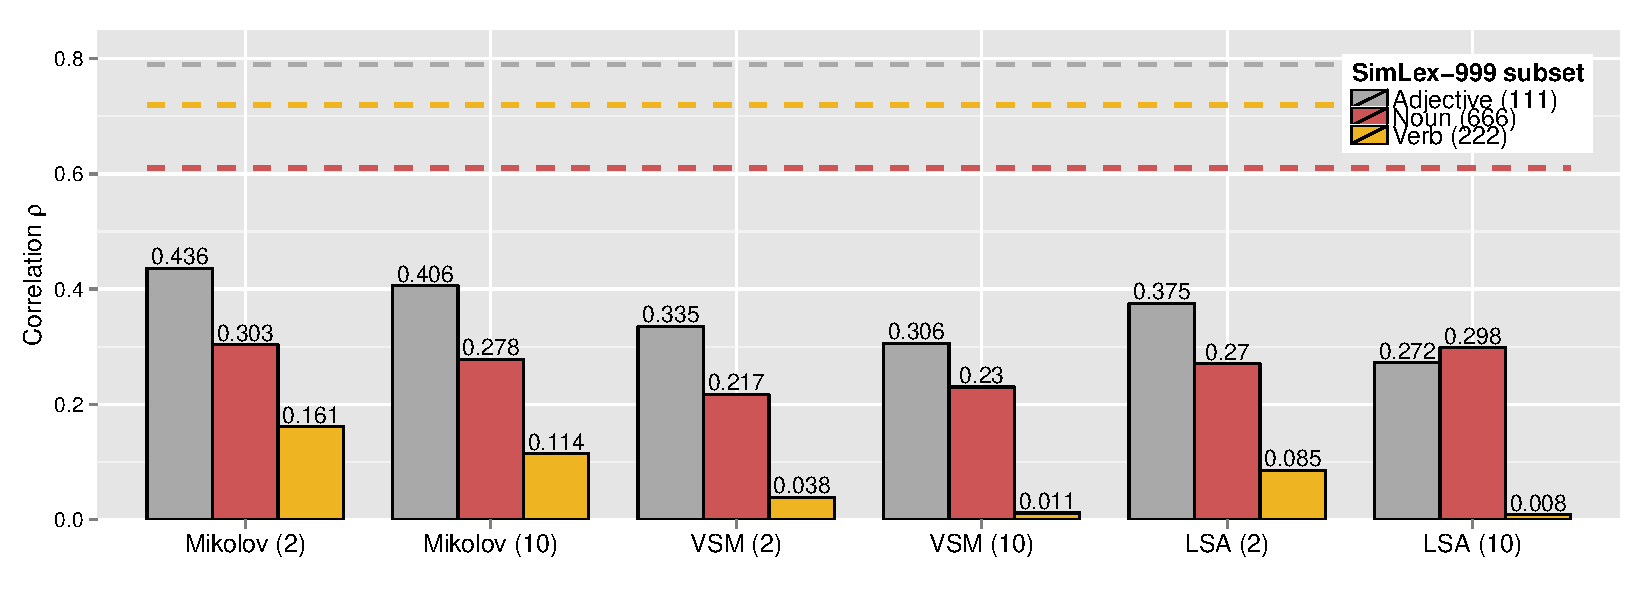
\includegraphics[width = \textwidth,height=5cm]{Chapter_3/Figure_5_CL}  \caption{Performance of models on POS-based subsets of SimLex-999. The window size for each model is indicated in parentheses. Inter-annotator agreement for each POS is indicated by the dashed horizontal line.}\end{figure*}

\begin{figure}[]  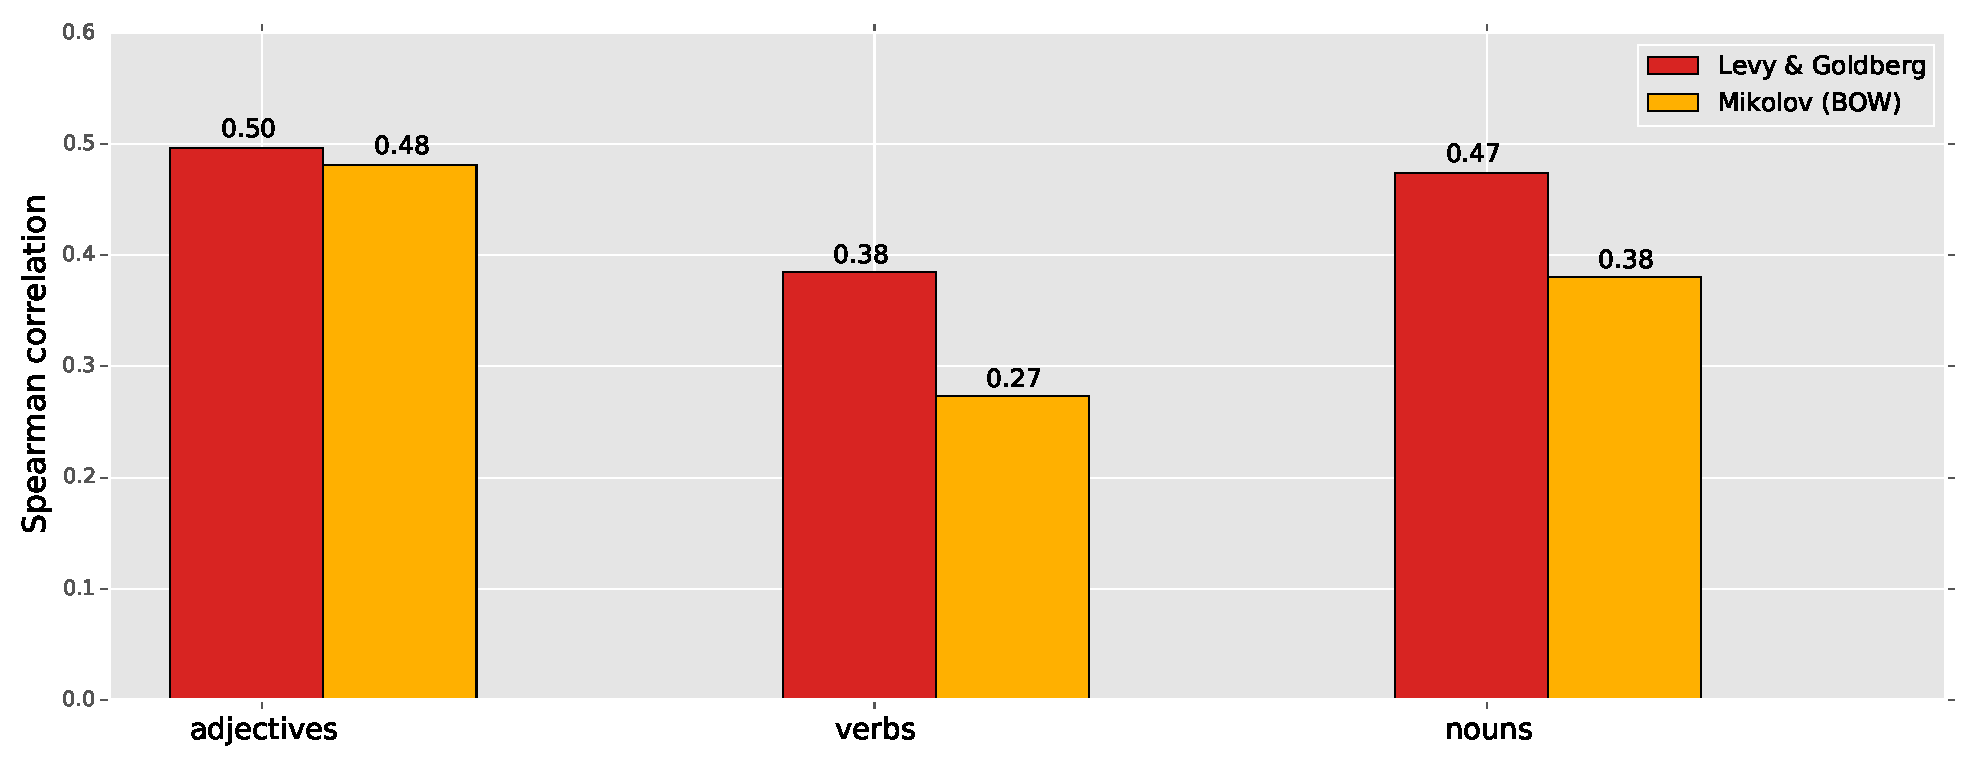
\includegraphics[width = \textwidth,height=5cm]{Chapter_3/New_Figure_2_CL}  \caption{The importance of dependency-focussed contexts (in the Levy \& Goldberg model) for capturing concepts of different POS, when compared to a standard Skipgram (BOW) model trained on the same Wikipedia corpus.}\end{figure}



\paragraph{\bf Learning concepts of different POS}

Given the theoretical likelihood of variation in model performance across POS categories noted in Section 2.2, we evaluated the \cite{mikolov2013efficient}, VSM and SVD models on the subsets of SimLex-999 containing adjective, noun and verb concept pairs. 

The analyses yield two notable conclusions, as shown in Figure 11. First, perhaps contrary to intuition, all models estimate the similarity of adjectives better than other concept categories. This aligns with the (also unexpected) observation that humans rate the similarity of adjectives more consistently and with more agreement than other parts of speech (see the dashed lines). However, the parallels between human raters and the models do not extend to verbs and nouns; verb similarity is rated more consistently than noun similarity by humans, but models estimate these ratings more accurately for nouns than for verbs. 

To better understand the linguistic information exploited by models when acquiring concepts of different POS, we also computed performance on the POS subsets of SimLex-999 of the dependency-based model of \cite{levy2014dependency} and the standard skipgram model, in which linguistic contexts are encoded as simple bags-of-words (BOW) \cite{mikolov2013efficient} (trained on the same Wikipedia text). As shown in Figure 12, dependency-aware contexts yield the largest improvements for capturing verb similarity. This aligns with the cognitive theory of verbs as \emph{relational concepts} \cite{markman1997similar} whose meanings rely on their interaction with (or dependency on) other words or concepts. It is also consistent with research on the automatic acquisition of verb semantics, in which syntactic features have proven particularly important \cite{sun2008verb}.  While a deeper exploration of these effects is beyond the scope of this work, this preliminary analysis again highlights the how the word classes integrated into SimLex-999 are pertinent to a range of questions concerning lexical semantics. 



\paragraph{\bf Learning concrete and abstract concepts}

\begin{figure*}[ht]  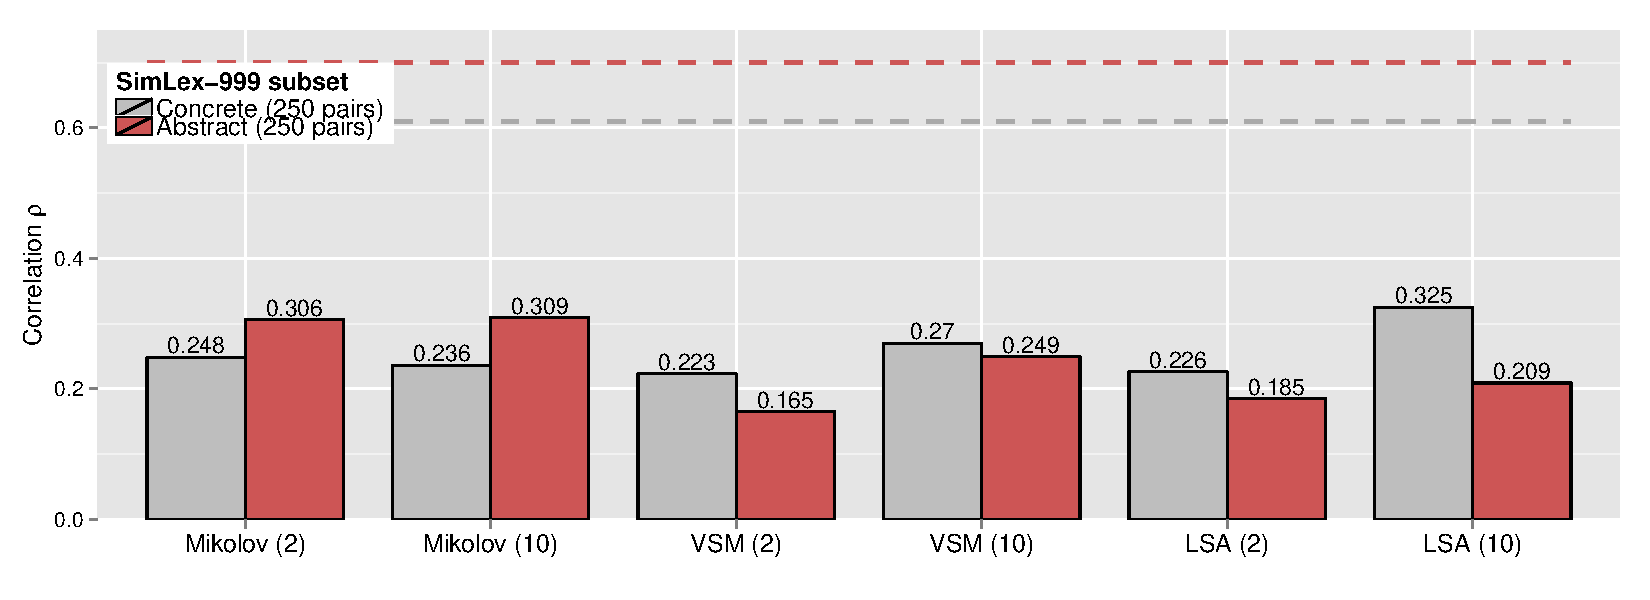
\includegraphics[width = \textwidth,height=5cm]{Chapter_3/Figure_4_CL}  \caption{Performance of models on concreteness-based subsets of SimLex-999. Window size is indicated in parentheses. Horizontal dashed lines indicate inter-annotator agreement between SimLex-999 annotators on the two subsets.}\end{figure*}


Given the strong interdependence between POS and conceptual concreteness (Figure 1), we aimed to explore whether the variation in model performance on different POS categories was in fact driven by an underlying effect of concreteness. To do so, we	 ranked each pair in the SimLex-999 dataset according to the sum of the concreteness of the two words, and compared performance of models on the most concrete and least concrete quartiles according to this ranking (Figure 13). 

Interestingly, the performance of models on the most abstract and most concrete pairs suggests that the distinction characterised by concreteness is at least partially independent of POS. Specifically, while the Mikolov et al. model was the highest performer on all POS categories, its performance was worse than both the simple VSM and SVD models (of window size 10) on the most concrete concept pairs.

This finding supports the growing evidence for systematic differences in representation and/or similarity operations between abstract and concrete concepts \cite{hill2013concreteness}, and suggests that at least part of these concreteness effects are independent of POS. In particular, it appears that models built from underlying vectors of co-occurrence counts, such as VSMs and SVD, are better equipped to capture the semantics of concrete entities, whereas the embeddings learned by NLMs can better capture abstract semantics. 

\section{Conclusion} 

Although the ultimate test of semantic models should be their utility in downstream applications, the research community can undoubtedly benefit from ways to evaluate the general quality of the representations learned by such models, prior to their integration in any particular system. We have presented SimLex-999, a gold standard resource for the evaluation of semantic representations containing similarity ratings of word pairs of different POS categories and concreteness levels. 

The development of SimLex-999 was principally motivated by two factors. First, as we demonstrated, several existing gold standards measure the ability of models to capture association rather than similarity, and others do not adequately test their ability to discriminate similarity from association. This is despite the many potential applications for accurate similarity-focussed representation learning models. Analysis of the ratings of the 500 SimLex-999 annotators showed that subjects can consistently quantify similarity, as distinct from association, and apply it to various concept types, based on minimal intuitive instructions. 

Second, as we showed, state-of-the-art models trained solely on running-text corpora have now reached or surpassed the human agreement ceiling on WordSim-353 and MEN, the most popular existing gold standards, as well as on RG and WS-Sim. These evaluations may therefore have limited use in guiding or moderating future improvements to distributional semantic models. Nevertheless, there is clearly still room for improvement in terms of the use of distributional models in functional applications. We therefore consider the comparatively low performance of state-of-the-art models on SimLex-999 to be one of its principal strengths. There is clear room under the inter-rating ceiling to guide the development of the next generation of distributional models. 

We conducted a brief exploration of how models might improve on this performance, and verified the hypotheses that models trained on dependency-based input capture similarity more effectively than those trained on running-text input. The evidence that smaller context windows are also beneficial for similarity models was mixed, however. Indeed, we showed that the optimal window size depends on both the general model architecture and the part-of-speech and concreteness of the target concepts. 

Our analysis of these hypotheses illustrates how the design of SimLex-999 - covering a principled set of concept categories and including meta-information on concreteness and free-association strength - enables fine-grained analyses of the performance and parameterization  of semantic models. However, these experiments only scratch the surface in terms of the possible analyses. We hope that researchers will adopt the resource as a robust means of answering a diverse range of questions pertinent to similarity modelling, distributional semantics and representation learning in general.  

In particular, for models to learn high-quality representations for all linguistic concepts, we believe that future work must uncover ways to explicitly or implicitly infer `deeper', more general, conceptual properties such as intentionality, polarity, subjectivity or concreteness \cite{gershmanmetaphor}. However, while improving corpus-based models in this direction is certainly realistic, models that learn exclusively via the linguistic modality may never reach human-level performance on evaluations such as SimLex-999. This is because much conceptual knowledge, and particularly that which underlines similarity computations for concrete concepts, appears to be grounded in the perceptual modalities as much as in language \cite{barsalou2003grounding}. 

Whatever the means by which the improvements are achieved, accurate concept-level representation is likely to constitute a necessary first step towards learning informative, language-neutral phrasal and sentential representations. Such representations would be hugely valuable for fundamental NLP applications such as language understanding tools and machine translation. 

Distributional semantics aims to infer the meaning of words based on the \emph{company they keep} \cite{dist}. However, while words that occur together in text often have associated meanings, these meanings may be very similar or indeed very different. Thus, possibly excepting the population of Argentina, most people would agree that, strictly speaking, \emph{Maradona} is not synonymous with \emph{football} (despite their high rating of 8.62 in WordSim-353). The challenge for the next generation of distributional models may therefore be to infer what is useful from the co-occurrence signal and to overlook what is not. Perhaps only then will models capture most, or even all, of what humans know when they know how to use a language. 

% include your own bib file like this:


\section{Sequence-to-Sequence Learning of Word Representations From Bilingual Data}


It is well known that word representations can be learned from the distributional patterns in corpora. Originally, such representations were constructed by counting word co-occurrences, so that the features in one word's representation corresponded to other words~\cite{landauer1997solution,turney2010frequency}. Neural language models, an alternative method for learning word representations, use language data to optimise (latent) features with respect to a language modelling objective. The objective can be to predict either the next word given the initial words of a sentence~\cite{Bengio2003lm,mnih2009scalable,collobert2008unified}, or simply a nearby word given a single cue word~\cite{mikolov2013distributed,Pennington2014}. The representations learned by neural models (sometimes called \emph{embeddings}) perform very effectively when applied as pre-trained features in a range of NLP applications and tasks~\cite{baroni2014don}. 

Despite these clear results, it is not well understood how the architecture of neural models affects the information encoded in their embeddings. Here we contribute to this understanding by considering the embeddings learned by architectures with a very different objective function: \emph{neural machine translation} (NMT) \emph{models}. NMT models have recently emerged as an alternative to statistical, phrase-based translation models, and are beginning to achieve impressive translation performance~\cite{kalchbrenner13emnlp,devlin2014fast,Sutskever2014sequence}.

We show that NMT models are not only a potential new direction for machine translation, but are also an effective means of learning word embeddings. Specifically, translation-based embeddings encode information relating to conceptual similarity (rather than non-specific relatedness or association) and lexical syntactic role more effectively than embeddings from monolingual neural language models. We demonstrate that these properties persist when translating between different language pairs (English-French and English-German). Further, based on the observation of subtle language-specific effects in the embedding spaces, we conjecture as to why similarity dominates over other semantic relations in translation embedding spaces. Finally, we discuss a potential limitation of the application of NMT models for embedding learning - the computational cost of training large vocabularies of embeddings - and show that a novel method for overcoming this issue preserves the aforementioned properties of translation-based embeddings. 

% We show that the precise information encoFinally, we consider ways to combine the distinct information encoded in language-model embeddings and those from translation embeddings. And we consider ways to overcome two important limitations of neural translation models as embedding-learning architectures: the computational difficulty in learning large vocabularies of embeddings, and the requirement for sentence-aligned bilingual training corpora.   

\section{Learning Embeddings with Neural Language Models}

All neural language models, including NMT models, learn real-valued embeddings (of specified dimension) for words in some pre-specified vocabulary, \(V\), covering many or all words in their training corpus. At each training step, a `score' for the current training example (or batch) is computed based on the embeddings in their current state. This score is compared to the model's objective function, and the error is backpropagated to update both the model weights (affecting how the score is computed from the embeddings) and the embedding features themselves. At the end of this process, the embeddings should encode information that enables the model to optimally satisfy its objective.     

\subsection{Monolingual Models}

In the original neural language model~\cite{Bengio2003lm} and subsequent
variants \cite{collobert2008unified}, training examples consist of an ordered sequence of $n$ words,
with the model trained to predict the $n$-th word given the first $n-1$
words. The model first represents the input as an ordered sequence of embeddings,
which it transforms into a single fixed length `hidden' representation, generally by concatenation and non-linear projection.
Based on this representation, a probability distribution is
computed over the vocabulary, from which the model can sample a guess for the
next word. The model weights and embeddings are updated to maximise the
probability of correct guesses for all sentences in the
training corpus. 
 
More recent work has shown that high quality word embeddings can be learned via simpler models
with no nonlinear hidden layer ~\cite{mikolov2013distributed,Pennington2014}. Given a single word or unordered window of words in the corpus, these models predict which words will occur nearby. For each word \( w\) in \(V\), a list of training cases \({(w,c) : c \in V }\) is extracted from the training corpus according to some algorithm.  For instance, in the \emph{skipgram}
approach ~\cite{mikolov2013distributed}, for each `cue word' \(w\) the `context words' \(c\) are sampled
from windows either side of tokens of \(w\) in the corpus (with \(c\) more
likely to be sampled if it occurs closer to \(w\)).\footnote{
    Subsequent variants use different algorithms for selecting the
    \((w,c)\) from the training corpus \cite{Hill2014EMNLP,levy2014dependency}
} For each \(w\) in \( V\), the model initialises both a
cue-embedding, representing the \(w\) when it occurs as a cue-word, and a
context-embedding, used when \(w\) occurs as a context-word. For a cue word
\(w\), the model uses the corresponding cue-embedding and all
context-embeddings to compute a probability distribution over \(V\) that
reflects the probability of a word occurring in the context of \(w\). When a
training example \((w,c)\) is observed, the model updates both the cue-word
embedding of \(w\) and the context-word embeddings in order to increase the
conditional probability of \(c\). 

\subsection{Bilingual Representation-learning Models}
Various studies have demonstrated that word representations can also be effectively learned from bilingual corpora, aligned at the document, paragraph or word level~\cite{Haghighi2008Learning,vulic2011identifying,mikolov2013exploiting,Hermann:2014:ICLR,lauly2014autoencoder}. These approaches aim to represent the words from two (or more) languages in a common vector space so that words in one language are close to words with similar or related meanings in the other. The resulting multilingual embedding spaces have been effectively applied to bilingual lexicon extraction~\cite{Haghighi2008Learning,vulic2011identifying,mikolov2013exploiting} and document classification~\cite{Klementiev,Hermann:2014:ICLR,lauly2014autoencoder,Kocisky:2014}.

We focus our analysis on two representatives of this class of (non-NMT) bilingual model. The first is that of \cite{Hermann:2014:ICLR}, whose embeddings improve on the performance of~\cite{Klementiev} in document classification applications. As with the NMT models introduced in the next section, this model can be trained directly on bitexts aligned only at the sentence rather than word level. When training, for aligned sentences \(S_E\) and \(S_F\) in different languages, the model computes representations \(R_E\) and \(R_F\) by summing the embeddings of the words in \(S_E\) and \(S_F\) respectively. The embeddings are then updated to minimise the divergence between \(R_E\) and \(R_F\) (since they convey a common meaning). A noise-contrastive loss function ensures that the model does not arrive at trivial (e.g. all zero) solutions to this objective.~\cite{Hermann:2014:ICLR} show that, despite the lack of prespecified word alignments, words in the two languages with similar meanings converge in the bilingual embedding space.\footnote{The models of \cite{lauly2014autoencoder} and \cite{Hermann:2014:ICLR} both aim to minimise the divergence between source and target language sentences represented as sums of word embeddings. Because of these similarities, we do not compare with both in this paper.}

The second model we examine is that of \cite{faruqui2014improving}. Unlike the models described above, \cite{faruqui2014improving} showed explicitly that projecting word embeddings from two languages (learned independently) into a common vector space can favourably influence the orientation of word embeddings when considered in their monolingual subspace; i.e relative to other words in their own language.  In contrast to the other models considered in this paper, the approach of \cite{faruqui2014improving} requires bilingual data to be aligned at the word level.

\subsection{Neural Machine Translation Models}

The objective of NMT is to generate an appropriate sentence in a target
language \(S_t\)  given a sentence \(S_s\) in the source language (see e.g.~\cite{kalchbrenner13emnlp,Sutskever2014sequence}). As a by-product of learning to meet this objective, NMT models learn distinct sets of embeddings for the vocabularies \(V_ s\) and \(V_t\) in the source and target languages respectively.

Observing a training case \((S_s, S_t)\), these models represent \(S_s\) as an ordered sequence of embeddings of words from \(V_s\). The sequence for \(S_s\) is then encoded into a single representation \(R_S\).\footnote{Alternatively, subsequences (phrases) of \(S_s\) may be encoded at this stage in place of the whole sentence~\cite{bahdanau2014neural}.} Finally, by referencing the embeddings in \(V_t\), \(R_S\) and a representation of what has been generated thus far, the model decodes a sentence in the target language word by word. If at any stage the decoded word does not match the corresponding word in the training target \(S_t\), the error is recorded. The weights and embeddings in the model, which together parameterise the encoding and decoding process, are updated based on the accumulated error once the sentence decoding is complete. 

Although NMT models can differ in their low-level architecture~\cite{kalchbrenner13emnlp,Cho2014,bahdanau2014neural}, the translation objective exerts similar pressure on the embeddings in all cases. The source language embeddings must be such that the model can combine them to form single representations for ordered sequences of multiple words (which in turn must enable the decoding process). The target language embeddings must facilitate the process of decoding these representations into correct target-language sentences.    

\section{Experiments}

To learn translation-based embeddings, we trained two different NMT models. The first is the RNN encoder-decoder, \emph{RNNenc}~\cite{Cho2014}, which uses a recurrent-neural-network to encode all of the source sentence into a single vector on which the decoding process is conditioned. The second is the \emph{RNN Search} architecture~\cite{bahdanau2014neural}, which was designed to overcome limitations exhibited by the RNN encoder-decoder when translating very long sentences. RNN Search includes a \emph{attention} mechanism, an additional feed-forward network that learns to attend to different parts of the source sentence when decoding each word in the target sentence.\footnote{Access to source code and limited GPU time prevent us from training and evaluating the embeddings from other NMT models such as that of~\cite{kalchbrenner13emnlp},~\cite{devlin2014fast} and \cite{Sutskever2014sequence}. The underlying principles of encoding-decoding also apply to these models, and we expect the embeddings would exhibit similar properties to those analysed here.} Both models were trained on a 348m word corpus of English-French sentence pairs or a 91m word corpus of English-German sentence pairs.\footnote{These corpora were produced from the WMT ’14 parallel data after conducting the data-selection procedure described by~\cite{Cho2014}. } 

To explore the properties of bilingual embeddings learned via objectives other than direct translation, we trained the \emph{BiCVM} model of~\cite{Hermann:2014:ICLR} on the same data, and also downloaded the projected embeddings of~\cite{faruqui2014improving}, \emph{FD}, trained on a bilingual corpus of comparable size (\(\approx 300\) million words per language).\footnote{Available from \url{http://www.cs.cmu.edu/~mfaruqui/soft.html}. The available embeddings were trained on English-German aligned data, but the authors report similar to for English-French.} Finally, for an initial comparison with monolingual models, we trained a conventional skipgram model~\cite{mikolov2013distributed} and its \emph{Glove} variant~\cite{Pennington2014} for the same number of epochs on the English half of the bilingual corpus. 

To analyse the effect on embedding quality of increasing the quantity of training data, we then trained the monolingual models on increasingly large random subsamples of Wikipedia text (up to a total of 1.1bn words). Lastly, we extracted embeddings from a full-sentence language model, \emph{CW},~\cite{collobert2008unified}, which was trained for several months on the same Wikipedia 1bn word corpus. Note that increasing the volume of training data for the bilingual (and NMT) models was not possible because of the limited size of available sentence-aligned bitexts. 
 
\subsection{Similarity and relatedness modelling}

As in previous studies~\cite{Agirre2009,bruni2014multimodal,baroni2014don}, our initial evaluations involved calculating pairwise (cosine) distances between embeddings and correlating these distances with (gold-standard) human judgements of the strength of relationships between concepts. For this we used three different gold standards: WordSim-353~\cite{Agirre2009}, MEN~\cite{bruni2014multimodal} and SimLex-999~\cite{hill2014simlex}. Importantly, there is a clear distinction between WordSim-353 and MEN, on the one hand, and SimLex-999, on the other, in terms of the semantic relationship that they quantify. For both WordSim-353 and MEN, annotators were asked to rate how \emph{related} or \emph{associated} two concepts are. Consequently, pairs such as [\emph{clothes}-\emph{closet}], which are clearly related but ontologically dissimilar, have high ratings in WordSim-353 and MEN. In contrast, such pairs receive a low rating in SimLex-999, where only genuinely \emph{similar} concepts, such as [\emph{coast}- \emph{shore}], receive high ratings. 

To reproduce the scores in SimLex-999, models must thus distinguish pairs that are similar from those that are merely related. In particular, this requires models to develop sensitivity to the distinction between synonyms (similar) and antonyms (often strongly related, but highly dissimilar).\footnote{For a more detailed discussion of the similarity/relatedness distinction, see~\cite{hill2014simlex}.}

Table~\ref{table:perf} shows the correlations of NMT (English-French) embeddings, other bilingually-trained embeddings and monolingual embeddings with these three lexical gold-standards. NMT outperform monolingual embeddings, and, to a lesser extent, the other bilingually trained embeddings, on SimLex-999. However, this clear advantage is not observed on MEN and WordSim-353, where the projected embeddings of~\cite{faruqui2014improving}, which were tuned for high performance on WordSim-353, perform best. Given the aforementioned differences between the evaluations, this suggests that bilingually-trained embeddings, and NMT based embeddings in particular, better capture similarity, whereas monolingual embedding spaces are orientated more towards relatedness. 

\begin{table}[t]
\begin{center}
\begin{tabular}{r c | r  r  r  | r r | r r |}
\multicolumn{2}{c|}{~} &\multicolumn{3}{c|}{Monolingual models}  & \multicolumn{2}{c|}{\small Biling. models} & \multicolumn{2}{c|}{NMT models}\\  
    \multicolumn{2}{c|}{~} &\bf Skipgram &\bf Glove &\bf CW & \bf FD & \bf BiCVM & \bf RNNenc &\bf RNNsearch \\ 
\hline
WordSim-353   & \(\rho\) & 0.52 & 0.55 & 0.51 &{\bf  0.69} & 0.50 &   0.57 &  0.58 \\
MEN & \(\rho\) & 0.44 & 0.71 & 0.60 & {\bf 0.78} & 0.45 &  0.63 &  0.62  \\
\hdashline
SimLex-999 & \(\rho\) & 0.29 & 0.32 & 0.28 & 0.39 & 0.36 &   {\bf 0.52} &  0.49 \\
SimLex-333 & \(\rho\) &  018&0.18  &0.07  & 0.24  &  0.34 & { \bf 0.49}   & 0.45   \\
TOEFL & \(\%\) & 0.75 & 0.78 & 0.64 & 0.84 & 0.87 &  {\bf 0.93} &  {\bf 0.93} \\
Syn/antonym & \(\%\) & 0.69  & 0.72  &  0.75 & 0.76 & 0.70 &  {\bf 0.79} & 0.74 \\
\end{tabular}
\caption{ NMT embeddings (RNNenc and RNNsearch) clearly outperform alternative embedding-learning architectures on tasks that require modelling similarity (below the dashed line), but not on tasks that reflect relatedness. Bilingual embedding spaces learned without the translation objective are somewhere between these two extremes.}
\label{table:perf}
\end{center}
\vspace{-5mm}
\end{table}


\begin{table}[t]
\begin{center}
\begin{tabular}{r | r  r  r | r r | r r}
&\bf Skipgram &\bf Glove &\bf CW&\bf FD &\bf BiCVM  &\bf RNNenc &\bf RNNsearch \\ 
\hline
\emph{teacher}  & {\small \emph{vocational}} &  {\small \emph{student}} 
& {\small \emph{student}} &{\small \emph{elementary}} & {\small  \emph{faculty}} & {\small \emph{professor}}  & {\small \emph{instructor}} \\ 
 & {\small \emph{in-service}} &  {\small \emph{pupil}} 
& {\small \emph{tutor}} & {\small \emph{school}}& {\small  \emph{professors}} & {\small \emph{instructor}}  & {\small \emph{professor}} \\ 
 & {\small \emph{college}} &  {\small \emph{university}} 
& {\small \emph{mentor}} & {\small \emph{classroom}}& {\small \emph{teach}}& {\small \emph{trainer}}  & {\small \emph{educator}} \\ 
\hdashline
\emph{eaten}  & {\small \emph{spoiled}} &  {\small \emph{cooked}} 
&  {\small \emph{baked}} &{\small \emph{ate}}& {\small  \emph{eating}}& {\small \emph{ate}} & {\small \emph{ate}} \\ 
  & {\small \emph{squeezed}} &  {\small \emph{eat}} 
&  {\small \emph{peeled}} &{\small \emph{meal}}& {\small \emph{eat}}& {\small \emph{consumed}} & {\small \emph{consumed}} \\ 
  & {\small \emph{cooked}} &  {\small \emph{eating}} 
&  {\small \emph{cooked}} &{\small \emph{salads}}& {\small \emph{baking}}& {\small \emph{tasted}} & {\small \emph{eat}} \\ 
\hdashline
\emph{Britain}  & {\small \emph{Northern}} &  {\small \emph{Ireland}} 
& {\small \emph{Luxembourg}} &{\small \emph{UK}}& {\small \emph{UK}} & {\small  \emph{UK}} & {\small \emph{England}} \\ 
& {\small \emph{Great}} &  {\small \emph{Kingdom}} 
& {\small \emph{Belgium}} &{\small \emph{British}}& {\small \emph{British}} & {\small  \emph{British}} & {\small \emph{UK}} \\ 
 & {\small \emph{Ireland}} &  {\small \emph{Great}} 
& {\small \emph{Madrid}} &{\small \emph{London}}& {\small \emph{England}} & {\small  \emph{America}} & {\small \emph{Syria}} \\ 


\end{tabular}
\caption{Nearest neighbours (excluding plurals) in the embedding spaces of different models. All models were trained for 6 epochs on the translation corpus except CW and FD (as noted previously). NMT embedding spaces are oriented according to similarity, whereas embeddings learned by monolingual models are organized according to relatedness. The other bilingual model BiCVM also exhibits a notable focus on similarity.}
\label{table:neigh}
\end{center}
\vspace{-5mm}
\end{table}

To test this hypothesis further, we ran three more evaluations designed to probe the sensitivity of models to similarity as distinct from relatedness or association. In the first, we measured performance on SimLex-Assoc-333 ~\cite{hill2014simlex}. This evaluation comprises the 333 most related pairs in SimLex-999, according to an independent empirical measure of relatedness (free associate generation~\cite{nelson2004university}). Importantly, the pairs in SimLex-Assoc-333, while all strongly related, still span the full range of similarity scores.\footnote{The most dissimilar pair in SimLex-Assoc-333 is [\emph{shrink,grow}] with a score of 0.23. The highest is [\emph{vanish},\emph{disappear}] with 9.80.} Therefore, the extent to which embeddings can model this data reflects their sensitivity to the similarity (or dissimilarity) of two concepts, even in the face of a strong signal in the training data that those concepts are related.    

The TOEFL synonym test is another similarity-focused evaluation of embedding spaces. This test contains 80 cue words, each with four possible answers, of which one is a correct synonym~\cite{landauer1997solution}. We computed the proportion of questions answered correctly by each model, where a model's answer was the nearest (cosine) neighbour to the cue word in its vocabulary.\footnote{To control for different vocabularies, we restricted the effective vocabulary of each model to the intersection of all model vocabularies, and excluded all questions that contained an answer outside of this intersection.} Note that, since TOEFL is a test of synonym recognition, it necessarily requires models to recognise similarity as opposed to relatedness.  

Finally, we tested how well different embeddings enabled a supervised classifier to distinguish between synonyms and antonyms, since synonyms are necessarily similar and people often find antonyms, which are necessarily dissimilar, to be strongly associated. For 744 word pairs hand-selected as either synonyms or antonyms,\footnote{Available online at \url{http://www.cl.cam.ac.uk/~fh295/}.} we presented a Gaussian SVM with the concatenation of the two word embeddings. We evaluated accuracy using 10-fold cross-validation. 

As shown in Table~\ref{table:perf}, with these three additional similarity-focused tasks we again see the same pattern of results. NMT embeddings outperform other bilingually-trained embeddings which in turn outperform monolingual models. The difference is particularly striking on SimLex-Assoc-333, which suggests that the ability to discern similarity from relatedness (when relatedness is high) is perhaps the most clear distinction between the bilingual spaces and those of monolingual models. 

These conclusions are also supported by qualitative analysis of the various embedding spaces. As shown in Table~\ref{table:neigh}, in the NMT embedding spaces the nearest neighbours (by cosine distance) to concepts such as \emph{teacher} are genuine synonyms such as \emph{professor} or \emph{instructor}. The bilingual objective also seems to orientate the non-NMT embeddings towards semantic similarity, although some purely related neighbours are also oberved. In contrast, in the monolingual embedding spaces the neighbours of \emph{teacher} include  highly related but dissimilar concepts such as \emph{student} or \emph{college}. 

%\footnote{Readers can inspect nearest neighbours in each embedding space using our web demo.} 
 
\subsection{Importance of training data quantity}

In previous work, monolingual models were trained on corpora many times larger than the English half of our parallel translation corpus. Indeed, the ability to scale to large quantities of training data was one of the principal motivations behind the skipgram architecture~\cite{mikolov2013distributed}. To check if monolingual models simply need more training data to capture similarity as effectively as bilingual models, we therefore trained them on increasingly large subsets of Wikipedia.\footnote{We did not do the same for our translation models because sentence-aligned bilingual corpora of comparable size do not exist.} As shown in Figure~\ref{fig:size}, this is not in fact the case. The performance of monolingual embeddings on similarity tasks remains well below the level of the NMT embeddings and somewhat lower than the non-MT bilingual embeddings as the amount of training data increases. 

\begin{figure*}[h]
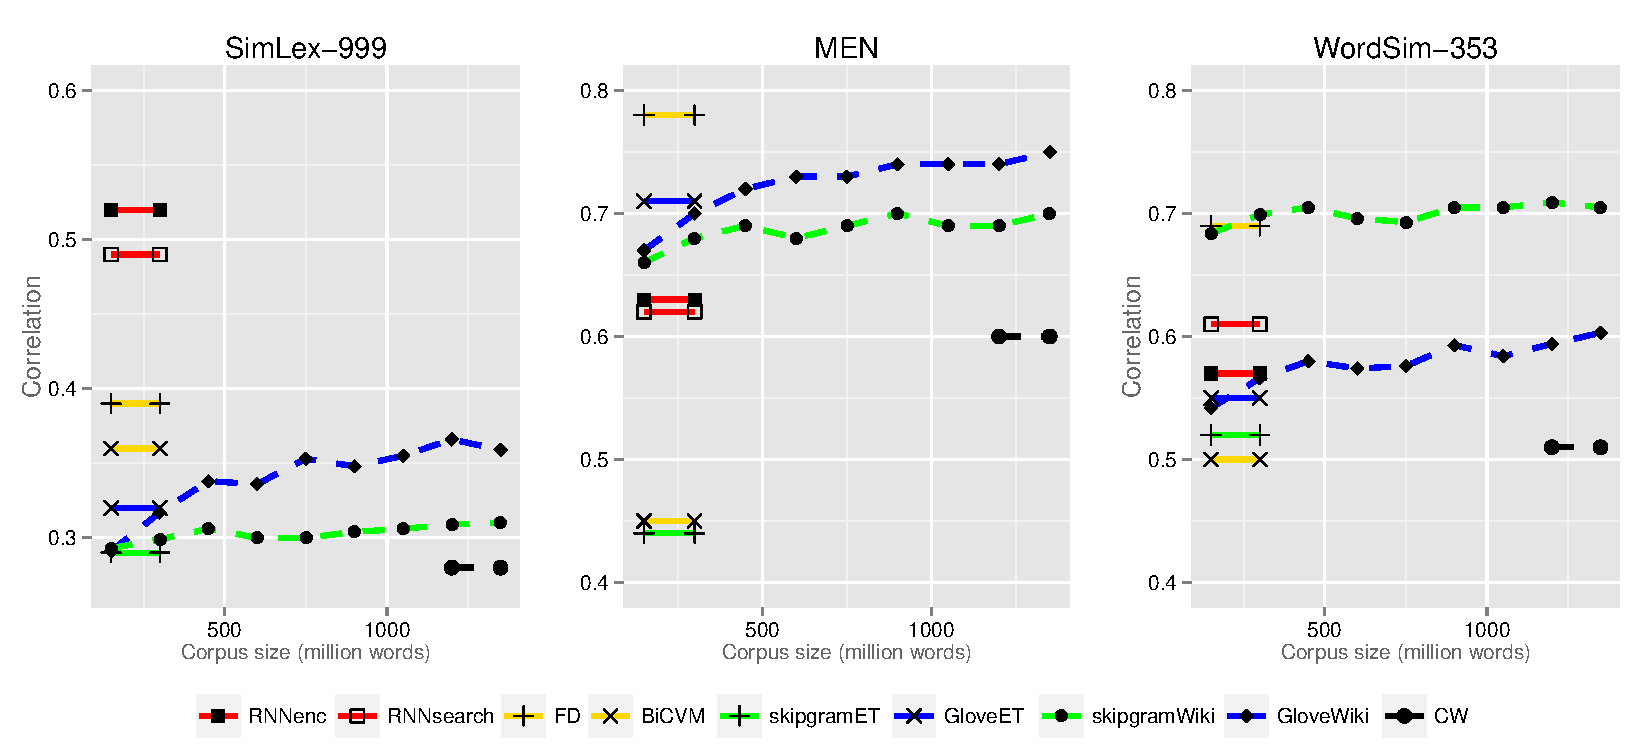
\includegraphics[width = \textwidth,clip=True,trim=0 10 0 10]{Chapter_3/Figure_1_ICLR2015}
\vspace{-4mm}
\caption{The effect of increasing the amount of training data on the quality of monolingual embeddings, based on similarity-based evaluations (SimLex-999) and two relatedness-based evaluations (MEN and WordSim-353). \emph{ET} in the legend indicates models trained on the English half of the translation corpus. \emph{Wiki} indicates models trained on Wikipedia.}
\label{fig:size}
\end{figure*}


\subsection{Analogy Resolution}

Lexical analogy questions have been used as an alternative way of evaluating word representations. In this task, models must identify the correct answer (\emph{girl}) when presented with analogy questions such as `\emph{man} is to \emph{boy} as \emph{woman} is to ?'. It has been shown that Skipgram-style models are surprisingly effective at answering such questions~\cite{mikolov2013distributed}. This is because, if \( \bf m, b \) and \( \bf w\) are skigram-style embeddings for \emph{man}, \emph{boy} and \emph{woman} respectively, the correct answer is often the nearest neighbour in the vocabulary (by cosine distance) to the vector \( \bf v = w + b - m \). 

We evaluated embeddings on analogy questions using the same vector-algebra method as~\cite{mikolov2013distributed}. As in the previous section, for fair comparison we excluded questions containing a word outside the intersection of all model vocabularies, and restricted all answer searches to this reduced vocabulary. This left 11,166 analogies. Of these, 7219 are classed as `syntactic', in that they exemplify mappings between parts-of-speech or syntactic roles (e.g. \emph{fast} is to \emph{fastest} as \emph{heavy} is to \emph{heaviest}), and 3947 are classed as `semantic` (\emph{Ottawa} is to \emph{Canada} as \emph{Paris} is to \emph{France}), since successful answering seems to rely on some (world) knowledge of the concepts themselves. 

As shown in Fig.~\ref{fig:analogy}, NMT embeddings yield relatively poor answers to semantic analogy questions compared with monolingual embeddings and the bilingual embeddings \emph{FD} (which are projections of similar monolingual embeddings).\footnote{The performance of the FD embeddings on this task is higher than that reported by~\cite{faruqui2014improving} because we search for answers over a smaller total candidate vocabulary.} It appears that the translation objective prevents the embedding space from developing the same linear, geometric regularities as skipgram-style models with respect to semantic organisation. This also seems to be true of the embeddings from the full-sentence language model \emph{CW}. Further, in the case of the Glove and FD models this advantage seems to be independent of both the domain and size of the training data, since embeddings from these models trained on only the English half of the translation corpus still outperform the translation embeddings. 

On the other hand, NMT embeddings are effective for answering syntactic analogies using the vector algebra method. They perform comparably to or even better than monolingual embeddings when trained on less data (albeit bilingual data). It is perhaps unsurprising that the translation objective incentivises the encoding of a high degree of lexical syntactic information, since coherent target-language sentences could not be generated without knowledge of the parts-of-speech, tense or case of its vocabulary items. The connection between the translation objective and the embedding of lexical syntactic information is further supported by the fact that embeddings learned by the bilingual model BiCVM do not perform comparably on the syntactic analogy task. In this model, sentential semantics is transferred via a bag-of-words representation, presumably rendering the precise syntactic information less important.

When considering the two properties of NMT embeddings highlighted by these experiments, namely the encoding of semantic similarity and lexical syntax, it is worth noting that items in the similarity-focused evaluations of the previous section (SimLex-999 and TOEFL) consist of word groups or pairs that have identical syntactic role. Thus, even though lexical semantic information is in general pertinent to conceptual similarity~\cite{levy2014dependency}, the lexical syntactic and conceptual properties of translation embeddings are in some sense independent of one another.  


\begin{figure*}[ht]

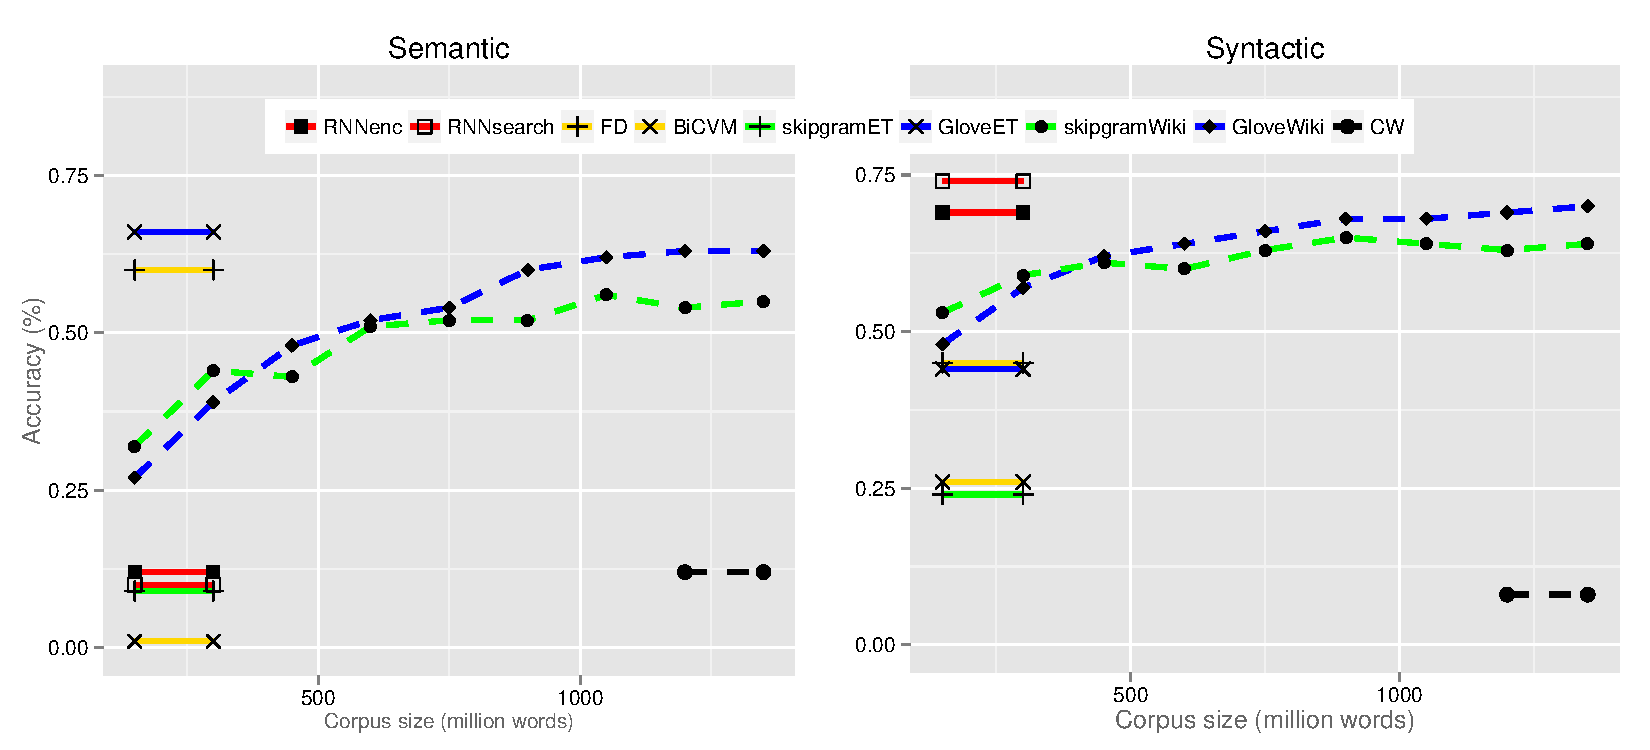
\includegraphics[width = \textwidth,clip=True,trim=0 10 0 10]{Chapter_3/Figure_2_ICLR2015}

\vspace{-4mm}
\caption{Translation-based embeddings perform best on syntactic analogies (\emph{run,ran: hide, hid}). Monolingual skipgram/Glove models are better at semantic analogies (\emph{father, man; mother, woman})}
\label{fig:analogy}

\end{figure*}

\section{Effect of Target Language}
\label{lang_effects}

To better understand why a translation objective yields embedding spaces with particular properties, we trained the RNN Search architecture to translate from English to German. 

\begin{table}[ht]
\begin{center}
\begin{tabular}{r c | m{0.9cm}  m{0.9cm}  r c c c }
    \multicolumn{2}{c|}{~} &\bf  \small EN-FR &\bf  \small EN-DE &  &  `earned' & `castle' & `money'\\ 
\cline{1-4} \cline{6-8}
WordSim-353   & \(\rho\) & 0.60 & \bf 0.61 &   & {\small \emph{gained}} & {\small \emph{chateau}} & {\small \bf \emph{ silver}} \\
MEN & \(\rho\) & 0.61 & \bf 0.62 \bf & \bf \small  EN-FR  & {\small \bf \emph{won}} & {\small \emph{palace}} & {\small \emph{funds}} \\
SimLex-999 & \(\rho\) & 0.49 &  \bf 0.50 &  & {\small \emph{acquired}}  & {\small \emph{fortress}}  & {\small \emph{cash}} \\
\cline{6-8}
SimLex-Assoc-333 & \(\rho\) & 0.45  & \bf 0.47   &   &  &   \\
TOEFL & \(\%\) & 0.90 & \bf 0.93  & &  {\small \emph{gained}}&  {\small \emph{chateau}} &  {\small \emph{funds}} \\ 
Syn/antonym & \(\%\) & \bf 0.72 &  0.70  &  \bf \small EN-DE   &  {\small \emph{deserved}}    &  {\small \emph{palace}}    &  {\small \emph{cash}} \\ 
Syntactic analogies & \(\%\) & \bf 0.73 & 0.62   &  &  {\small \emph{accummulated}}   &  {\small \bf \emph{ padlock}}   &  {\small \emph{resources}} \\  
Semantic analogies & \(\%\) & 0.10 & \bf  0.11  \\
\end{tabular}
\caption{Comparison of embeddings learned by RNN Search models translating between English-French (EN-FR) and English-German (EN-DE) on all semantic evaluations (left) and nearest neighbours of selected cue words (right). Bold italics indicate target-language-specific effects. Evaluation items and vocabulary searches were restricted to words common to both models. }
\label{table:de}
\end{center}
\vspace{-5mm}
\end{table}

As shown in Table~\ref{table:de} (left side), the performance of the source (English) embeddings learned by this model was comparable to that of those learned by the English-to-French model on all evaluations, even though the English-German training corpus (91 million words) was notably smaller than the English-French corpus (348m words). This evidence shows that the desirable properties of translation embeddings highlighted thus far are not particular to English-French translation, and can also emerge when translating to a different language family, with different word ordering conventions.     

\section{Overcoming the Vocabulary Size Problem}

A potential drawback to using NMT models for learning word embeddings is the computational cost of training such a model on large vocabularies. To generate a target language sentence, NMT models repeatedly compute a softmax distribution over the target vocabulary. This computation scales with vocabulary size and must be repeated for each word in the output sentence, so that training models with large output vocabularies is challenging. Moreover, while the same computational bottleneck does not apply to the encoding process or source vocabulary, there is no way in which a translation model could learn a high quality source embedding for a word if the plausible translations were outside its vocabulary. Thus, limitations on the size of the target vocabulary effectively limit the scope of NMT models as representation-learning tools. This contrasts with the shallower monolingual and bilingual representation-learning models considered in this paper,  which efficiently compute a distribution over a large target vocabulary using either a hierarchical softmax~\cite{morin2005hierarchical} or approximate methods such as negative sampling~\cite{mikolov2013distributed,Hermann:2014:ICLR}, and thus can learn large vocabularies of both source and target embeddings.

A recently proposed solution to this problem enables NMT models to be trained with larger target vocabularies (and hence larger meaningful source vocabularies) at comparable computational cost to training with a small target vocabulary~\cite{Jean}. The algorithm uses (biased) importance sampling~\cite{Bengio+Senecal-2003-small} to approximate the probability distribution of words over a large target vocabulary with a finite set of distributions over subsets of that vocabulary. Despite this element of approximation in the decoder, extending the effective target vocabulary in this way significantly improves translation performance, since the model can make sense of more sentences in the training data and encounters fewer unknown words at test time. In terms of representation learning, the method provides a means to scale up the NMT approach to vocabularies as large as those learned by monolingual models. However, given that the method replaces an exact calculation with an approximate one, we tested how the quality of source embeddings is affected by scaling up the target language vocabulary in this way. 

\begin{table}[t]
\begin{center}
\begin{tabular}{r c | c c c c }
    \multicolumn{2}{c|}{~} &\bf RNN Search &\bf RNN Search & \bf RNN Search-LV  & \bf RNN Search-LV  \\ 
 \multicolumn{2}{c|}{~} &\bf \small EN-FR &\bf \small  EN-DE & \bf  \small EN-FR & \bf \small EN-DE \\ 
\hline
WordSim-353   & \(\rho\) & 0.60 & \bf 0.61 & 0.59 & 0.57  \\
MEN & \(\rho\) & 0.61 & \bf 0.62 & \bf 0.62 & 0.61 \\
SimLex-999 & \(\rho\) & 0.49 & 0.50 & \bf  0.51 & 0.50  \\
SimLex-Assoc-333 & \(\rho\) & 0.45  & \bf 0.47  & \bf 0.47  & 0.46   \\
TOEFL & \(\%\) & 0.90 & 0.93 & 0.93 & \bf 0.98  \\
Syn/antonym & \(\%\) & 0.72 &  0.70 & \bf 0.74 & 0.71 \\
Syntactic analogies & \(\%\) & \bf 0.73 &  0.62 & 0.71 & 0.62\\
Semantic analogies & \(\%\) & 0.10 &  0.11 & 0.08 & \bf 0.13\
\end{tabular}
\caption{Comparison of embeddings learned by the original (RNN Search - 30k French words, 50k German words) and extended-vocabulary (RNN Search-LV -500k words) models translating from English to French (EN-FR) and from English to German (EN-DE). For fair comparisons, all evaluations were restricted to the intersection of all model vocabularies.}
\label{table:ex}
\end{center}
\vspace{-5mm}
\end{table}

As shown in Table~\ref{table:ex}, there is no significant degradation of embedding quality when scaling to large vocabularies with using the approximate decoder. Note that for a fair comparison we filtered these evaluations to only include items that are present in the smaller vocabulary. Thus, the numbers do not directly reflect the quality of the additional 470k embeddings learned by the extended vocabulary models, which one would expect to be lower since they are words of lower frequency. All embeddings can be downloaded from \url{http://www.cl.cam.ac.uk/~fh295/}, and the embeddings from the smaller vocabulary models can be interrogated at \url{http://lisa.iro.umontreal.ca/mt-demo/embs/}.\footnote{A different solution to the rare-word problem was proposed by~\cite{luong2014addressing}. We do not evaluate the effects on the resulting embeddings of this method because we lack access to the source code.} 


\section{How Similarity Emerges}
\label{section:exp}

Although NMT models appear to encode both conceptual similarity and syntactic information for any source and target languages, it is not the case that embedding spaces will always be identical. Interrogating the nearest neighbours of the source embedding spaces of the English-French and English-German models reveals occasional language-specific effects. As shown in Table~\ref{table:de} (right side), the neighbours for the word \emph{earned} in the English-German model are as one might expect, whereas the neighbours from the English-French model contain the somewhat unlikely candidate \emph{won}. In a similar vein, while the neighbours of the word \emph{castle} from the English-French model are unarguably similar, the neighbours from the English-German model contain the word \emph{padlock}.
 
These infrequent but striking differences between the English-German and English-French source embedding spaces indicate how similarity might emerge effectively in NMT models. Tokens of the French verb \emph{gagner} have (at least) two possible English translations (\emph{win} and \emph{earn}). Since the translation model, which has limited encoding capacity, is trained to map tokens of \emph{win} and \emph{earn} to the same place in the target embedding space, it is efficient to move these concepts closer in the source space. Since \emph{win} and \emph{earn} map directly to two different verbs in German, this effect is not observed. On the other hand, the English nouns \emph{castle} and \emph{padlock} translate to a single noun (\emph{Schloss}) in German, but different nouns in French. Thus, \emph{padlock} and \emph{castle} are only close in the source embeddings from the English-German model. 

Based on these considerations, we can conjecture that the following condition on the semantic configuration between two language is crucial to the effective induction of lexical similarity. 

\MyQuote{\emph{For \(s_1\) and \(s_2\) in the source language, there is some \(t\) in the target language such that there are sentences in the training data in which \(s_1\) translates to \(t\) and sentences in which \(s_2\) translates to \(t\).}}

{\centering \emph{if and only if} \\}

\MyQuote{\emph{\(s_1\) and \(s_2\) are semantically similar.}}

Of course, this condition is not true in general. However, we propose that the extent to which it holds over all possible word pairs corresponds to the quality of similarity induction in the translation embedding space. Note that strong polysemy in the target language, such as \emph{gagner = win, earn}, can lead to cases in which \(1\) is satisfied but \(2\) is not. The conjecture claims that these cases are detrimental to the quality of the embedding space (at least with regards to similarity). In practice, qualitative analyses of the embedding spaces and native speaker intuitions suggest that such cases are comparatively rare. Moreover, when such cases are observed, \(s_1\) and \(s_2\), while perhaps not similar, are not strongly dissimilar. This could explain why related but strongly dissimilar concepts such as antonym pairs do not converge in the translation embedding space. This is also consistent with qualitative evidence presented by ~\cite{faruqui2014improving} that projecting monolingual embeddings into a bilingual space orientates them to better reflect the synonymy/antonymy distinction.
    

\section{Conclusion}

In this work, we have shown that the embedding spaces from neural machine translation models are orientated more towards conceptual similarity than those of monolingual models, and that translation embedding spaces also reflect richer lexical syntactic information. To perform well on similarity evaluations such as SimLex-999, embeddings must distinguish information pertinent to what concepts \emph{are} (their function or ontology) from information reflecting other non-specific inter-concept relationships. Concepts that are strongly related but dissimilar, such as antonyms, are particularly challenging in this regard~\cite{hill2014simlex}. Consistent with the qualitative observation made by ~\cite{faruqui2014improving}, we suggested how the nature of the semantic correspondence between the words in languages enables NMT embeddings to distinguish synonyms and antonyms and, more generally, to encode the information needed to reflect human intuitions of similarity.   

The language-specific effects we observed in Section~\ref{lang_effects} suggest a potential avenue for improving translation and multi-lingual embeddings in future work. First, as the availability of fast GPUs for training grows, we would like to explore the embeddings learned by NMT models that translate between much more distant language pairs such as English-Chinese or English-Arabic. For these language pairs, the word alignment will less monotonic and may result in even more important semantic and syntactic information being encoded in the lexical representation. Further,  as observed by both~\cite{Hermann:2014:ICLR} and~\cite{faruqui2014improving}, the bilingual representation learning paradigm can be naturally extended to update representations based on correspondences between multiple languages (for instance by interleaving English-French and English-German training examples). Such an approach should smooth out language-specific effects, leaving embeddings that encode only language-agnostic conceptual semantics and are thus more generally applicable. Another related challenge is to develop smaller or less complex representation-learning tools that encode similarity with as much fidelity as NMT models but without the computational overhead. One promising approach for this is to learn word alignments and word embeddings jointly~\cite{Kocisky:2014}. This approach is effective for cross-lingual document classification, although the authors do evaluate the monolingual subspace induced by the model.\footnote{These embeddings are not publicly available and we were unable to re-train them using the source code.}

Not all word embeddings learned from text are born equal. Depending on the application, those learned by NMT models may have particularly desirable properties. For decades, distributional semantic models have aimed to exploit Firth's famous \emph{distributional hypothesis} to induce word meanings from (monolingual) text. However, the hypothesis also betrays the weakness of the monolingual distributional approach when it comes to learning humah-quality concept representations. For while it is undeniable that ``words which are similar in meaning appear in similar distributional contexts"~\cite{dist}, the converse assertion, which is what really matters, is only sometimes true. 




